\documentclass[italian,a4paper,10pt]{article}
\usepackage[footnotesize,bf]{caption}
\usepackage{babel,amsmath,amssymb,amsthm,graphicx,url,array,wrapfig,subfig}
\usepackage[text={6in,9in},centering]{geometry}
\usepackage[utf8x]{inputenc}
\usepackage[usenames]{color}
\frenchspacing
\pagestyle{plain}
\captionsetup[subfloat]{labelformat=simple,listofformat=subsimple}
%------------- eliminare prime e ultime linee isolate
\clubpenalty=9999%
\widowpenalty=9999
%------------- impostazioni environment teoremi
\theoremstyle{definition}
\newtheorem{theorem}{Esercizio}
%\newtheorem{lemma}[theorem]{Lemma} % [theorem] usa lo stesso contatore dei teoremi
%\newtheorem{prop}[theorem]{Proposizione}
%\newtheorem{definition}[theorem]{Definizione}
%\newtheorem{corollary}[theorem]{Corollario}
%\newtheorem{notation}[theorem]{Notazione}
%
%
%--- definizione numerazioni
\renewcommand{\theequation}{\thetheorem.\arabic{equation}}
\renewcommand{\thefigure}{\thesection.\arabic{figure}}
\renewcommand{\thetable}{\thesection.\arabic{table}}
\renewcommand{\thesubtable}{\thetable.\arabic{subtable}}
\addto\captionsitalian{%
  \renewcommand{\figurename}%
{Grafico}%
}
%
%------------- ridefinizione simbolo per elenchi puntati: en dash
%\renewcommand{\labelitemi}{\textbf{--}}
\renewcommand{\labelenumi}{\textbf{(\roman{enumi})}}
\setlength{\abovecaptionskip}{\baselineskip}   % 0.5cm as an example
\setlength{\floatsep}{2\baselineskip}
\setlength{\belowcaptionskip}{\baselineskip}   % 0.5cm as an example
%------------- nuovi environment senza spazi
%\newenvironment{packed_item}{
%\begin{itemize}
%  \setlength{\itemsep}{1pt}
%  \setlength{\parskip}{0pt}
%  \setlength{\parsep}{0pt}
%}{\end{itemize}}
%\newenvironment{packed_enum}{
%\begin{enumerate}
%  \setlength{\itemsep}{1pt}
%  \setlength{\parskip}{0pt}
%  \setlength{\parsep}{0pt}
%}{\end{enumerate}}
%\newenvironment{packed_description}{
%\begin{enumerate}
%   \setlength{\itemsep}{1pt}
%   \setlength{\parskip}{0pt}
%   \setlength{\parsep}{0pt}
% }{\end{enumerate}}
%--------- comandi insiemi numeri complessi, naturali, reali e altre abbreviazioni
\newcommand{\e}{\mathrm{e}}
\newcommand{\epsi}{\varepsilon}
\newcommand{\eqnum}{\setcounter{equation}{0}}
\newcommand{\spazio}{\vspace{.5\baselineskip}\\}
\renewcommand{\textfraction}{0.05}
\renewcommand{\topfraction}{0.95}
\renewcommand{\bottomfraction}{0.95}
\renewcommand{\floatpagefraction}{0.35}
\setcounter{totalnumber}{5}
%---------
%
%---------
\begin{document}
\title{Relazione di Laboratorio: il pendolo}
\author{\normalsize Ilaria Brivio (582116)\\%
\normalsize \url{brivio.ilaria@tiscali.it}%
\and %
\normalsize Matteo Abis (584206)\\ %
\normalsize \url{webmaster@latinblog.org}}
\date{\today}
\maketitle
%------------------
\begin{table}[hpt]
 \begin{tabular}{l l}
  \emph{Corso:} &Esperimentazioni Fisica 1 -- LT, A.A. 2007--2008\\
  \emph{Docente:} &dott. Cinzia Sada\\
 \end{tabular}
\end{table}
\section{Obiettivo dell'esperienza}
L'obiettivo primario dell'esperienza è il confronto di vari metodi di raccolta di dati sperimentali e la loro analisi, con particolare attenzione alla stima del ``valor vero'' e degli errori casuali e sistematici, per stabilire quale possa essere il modo migliore per misurare il periodo di oscillazione del pendolo, a parità di condizioni e tempo a disposizione.
\section{Descrizione dell'apparato strumentale}
\renewcommand{\arraystretch}{1.2}
\begin{wrapfigure}[16]{r}{40mm}
  \begin{center}
    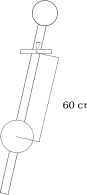
\includegraphics{disegno.jpg}
  \end{center}
  \caption{Rappresentazione schematica del pendolo.}\label{disegno}
\end{wrapfigure}
Lo strumento è un pendolo (vedi figura~\ref{disegno}), costituito da una barra di metallo a cui sono fissate due masse: una $60$~cm al di sotto del sostegno e un contrappeso al di sopra. Il pendolo oscilla su un coltello di acciaio temprato largo $5\cdot10^{-2}$~mm.

Nella prima parte dell'esperienza è stato utilizzato un cronometro manuale, con sensibilità di $10^{-3}$~s. Nella seconda parte, invece, il cronometro era dotato di un sistema di rilevazione automatico, ovvero una fotocellula sensibile al passaggio del pendolo nel punto più basso della traiettoria di oscillazione. Tale sistema ha una sensibiltà di $10^{-4}$~s ed è programmato in modo da registrare la durata di un periodo intero.
\section{Descrizione della metodologia di misura}
Sono stati registrati manualmente tre campioni di dati: un primo di 120 misure di una singola oscillazione completa (vedi tabella~\ref{tab100}), un secondo di 52 misure di due oscillazioni (vedi tabella~\subref{tab50}) e un terzo campione di 28 misure di quattro oscillazioni (vedi tabella~\subref{tab25}). Il tempo qui misurato come periodo è l'intervallo tra due arresti consecutivi del pendolo sullo stesso lato.

Con l'apparato automatico sono state raccolte prima 100, poi 999 misure. Il sistema rileva il tempo trascorso tra due passaggi consecutivi del pendolo nel punto più basso del suo movimento, ed è programmato per salvare dati relativi a un'oscillazione completa, e non ai semiperiodi.
\newpage
\section{Risultati sperimentali ed elaborazione dati}
I tempi registrati nei campioni sono riportati nelle tabelle successive. Per ogni campione è stato elaborato un istogramma suddividendo i dati in classi di frequenza dell'ampiezza di $15$~ms, messo a confronto con una distribuzione casuale gaussiana. Sono stati inoltre calcolati media aritmetica~$\bar{x}$, l'errore quadratico medio~$\sigma$ e l'errore della media~$\sigma_{\bar{x}}$. Nel campione relativo alle misure manuali della singola oscillazione, è stato individuato un valore esterno all'intervallo $[\bar{x} - 3\sigma,\bar{x} + 3\sigma]$ e quindi escluso.
\begin{table}[h!]\centering
\begin{tabular}{ c *3{r@{.}l}r@{ $\pm$ }l }
 \multicolumn{1}{ c }{n. misure $\times$ osc.}&
 \multicolumn{2}{c}{$\bar{x}$ (ms)}&
 \multicolumn{2}{c}{$\sigma$} &
 \multicolumn{2}{c}{$\sigma_{\bar{x}}$} &
 \multicolumn{2}{c}{risultato}\\
 \hline
 $120 \times 1$  	& 1936&47	&  63&64 	& 5&81 		&  1936.5  & 5.8\\
 $52 \times 2$  	& 3859&51 	&  88&07 	& 12&10 	&  3859.5  &12.1\\
 $28 \times 4$  	& 7711&79  	&   88&09  	&  16&65  	&   7711.8 &16.7\\
 $100$ (auto)		& 1927&21 	&  0&09 	& 0&01 		&  1927.21 &0.01\\
\end{tabular}
\end{table}\\
Ovvero, riportando i valori a un'oscillazione:
\begin{table}[h]\centering
\begin{tabular}{r r@{.}l @{ $\pm$ } r@{.}l @{ ms}}
120 & 1936&5 & 5&8 \\
52 & 1929&7 & 6&0  \\
28 & 1927&9 & 4&1  \\
100a & 1927&21 & 0&01  \\
\end{tabular}
\end{table}\\
\`{E} stata calcolata la compatibilità $\lambda$ di tali valori, secondo la formula:
\begin{equation*}
 \lambda_{i,j} = \dfrac{|\bar{x}_i - \bar{x}_j|}{\sqrt{\sigma_{\bar{x}_i}^2 + \sigma_{\bar{x}_j}^2}}
\end{equation*}
Con i seguenti risultati:
\begin{table}[h]\centering
\begin{tabular}{@{}r|r@{.}l r@{.}l r@{.}l}
 $\lambda$	&
 \multicolumn{2}{c}{120}
&   \multicolumn{2}{c}{52}
&   \multicolumn{2}{c}{28}  		\\
 \hline
 100a 		&  1&59 	&  0&42 	& 0&18 		\\
 28   		&  1&19 	&  0&25 	& \multicolumn{2}{c}{} \\
 52  	 	&  0&80 	& \multicolumn{2}{c}{}	& \multicolumn{2}{c}{}		 \\
\end{tabular}
\end{table}\\
La compatibilità si dice buona se ha valore compreso tra $0$ e $1$, mediocre tra~$1$~e~$2$~e scarsa tra~$2$~e~$3$.
I dati sono stati anche organizzati in istogrammi e confrontati con la curva gaussiana:
\begin{equation*}
 f(x) = \dfrac{N\Delta x}{\sigma \sqrt{2\pi}}\exp \left\{-\dfrac 1 2 \Big({\dfrac{x-\bar{x}}{\sigma}}\Big)^2\right\}
\end{equation*}
Dove $\Delta x$ è l'ampiezza delle classi di frequenza (15 ms), $N$ il numero totale di osservazioni e $\bar{x}$ la media aritmetica.
\section{Discussione dei risultati}
L'indice di compatibilità rispetto alle misure automatiche, gli errori sulle misure e sulla media mostrano chiaramente che la stima migliore è quella data dalle osservazioni su più periodi consecutivi. Ciò è giustificato dal fatto che l'errore $\sigma$ dovuto soprattutto al tempo di reazione dell'osservatore, è pressapoco costante su ogni misura, ma viene distribuito su un maggior numero di periodi, dunque influisce meno sulla stima della singola oscillazione. A conferma 

Per quanto riguarda i grafici, la distribuzione casuale degli errori è più evidente nelle misure di singole oscillazioni (come si vede dal grafico~\ref{gr1}) nonostante il picco sia spostato di circa 20~ms a destra. Il secondo grafico~(\ref{gr2}) rispetta meglio la stima centrale, anche se la scarsità di dati produce numerose irregolarità, che sono ancora più evidenti nel terzo istogramma~(\ref{gr4}) dove il picco di frequenza è quasi isolato. In tutti e tre i grafici si nota inoltre che la forma dell'istogramma presenta massimi secondari in eccesso di circa 50~ms.

Più interessante risulta il grafico delle 999 rilevazioni automatiche, in cui il massimo è nettamente spostato a sinistra e la distribuzione non è affatto simmetrica per la presenza di un errore sistematico dovuto all'approssimazione del periodo di oscillazione come indipendente dall'ampiezza dell'angolo. Una migliore approssimazione sarebbe infatti:
\begin{equation*}
 T = T_0\left(1+\dfrac{\alpha^2}{16}+\dfrac{9\alpha^4}{1024}+\cdots\right)
\end{equation*}
Come testimonia anche il grafico~\ref{gr1000} con le misure in ordine di rilevazione, il periodo diminuisce con lo smorzamento dell'oscillazione di circa 3~ms dopo 1000 periodi, ma non in modo lineare, ovvero in modo sempre meno marcato. Di conseguenza l'errore casuale è più evidente nelle ultime misure, che risultano più irregolari. Per lo stesso motivo l'istogramma delle frequenze si avvicina a una distribuzione casuale solo nella sua parte sinistra. Il grafico~\ref{sist} mostra una gaussiana con i dati di tutte le 999 misure, evidentemente inadeguata a rendere conto della distribuzione per la presenza dell'errore sistematico, mentre la gaussiana relativa ai dati delle ultime 500 osservazioni risulta meglio centrata sul massimo e più coerente con le misure intorno.

La serie di 999~misure automatiche è stato poi analizzato suddividendolo in dieci blocchi (vedi tabella~\ref{blocchi}), cosa che evidenzia ancora una volta la diminuzione della durata delle oscillazioni.

\section{Conclusioni}
L'esperienza dimostra chiaramente che per misurare manualmente il periodo di un pendolo è utile raggruppare più oscillazioni in una stessa misura, per distribuire l'effetto dell'imprecisione dovuta alla prontezza dell'operatore, che si può quantificare nell'ordine di grandezza di $10^{-1} s$. Una strumentazione elettronica permette invece di ridurre tali errori di tre ordini di grandezza rendendo possibile lo studio di errori sistematici dovuti allo smorzamento dell'ampiezza di oscillazione.
\newpage
\section{Appendice}
   \begin {figure}[hp]\caption{Campione di 120 misure di un'oscillazione.}\label{gr1}
      \begin{center}
        % GNUPLOT: LaTeX picture
\setlength{\unitlength}{0.240900pt}
\ifx\plotpoint\undefined\newsavebox{\plotpoint}\fi
\begin{picture}(1049,629)(0,0)
\sbox{\plotpoint}{\rule[-0.200pt]{0.400pt}{0.400pt}}%
\put(100,123){\makebox(0,0)[r]{ 0}}
\put(120.0,123.0){\rule[-0.200pt]{4.818pt}{0.400pt}}
\put(100,181){\makebox(0,0)[r]{ 2}}
\put(120.0,181.0){\rule[-0.200pt]{4.818pt}{0.400pt}}
\put(100,240){\makebox(0,0)[r]{ 4}}
\put(120.0,240.0){\rule[-0.200pt]{4.818pt}{0.400pt}}
\put(100,298){\makebox(0,0)[r]{ 6}}
\put(120.0,298.0){\rule[-0.200pt]{4.818pt}{0.400pt}}
\put(100,357){\makebox(0,0)[r]{ 8}}
\put(120.0,357.0){\rule[-0.200pt]{4.818pt}{0.400pt}}
\put(100,415){\makebox(0,0)[r]{ 10}}
\put(120.0,415.0){\rule[-0.200pt]{4.818pt}{0.400pt}}
\put(100,473){\makebox(0,0)[r]{ 12}}
\put(120.0,473.0){\rule[-0.200pt]{4.818pt}{0.400pt}}
\put(100,532){\makebox(0,0)[r]{ 14}}
\put(120.0,532.0){\rule[-0.200pt]{4.818pt}{0.400pt}}
\put(100,590){\makebox(0,0)[r]{ 16}}
\put(120.0,590.0){\rule[-0.200pt]{4.818pt}{0.400pt}}
\put(120,82){\makebox(0,0){ 1800}}
\put(120.0,123.0){\rule[-0.200pt]{0.400pt}{4.818pt}}
\put(157.0,123.0){\rule[-0.200pt]{0.400pt}{2.409pt}}
\put(194.0,123.0){\rule[-0.200pt]{0.400pt}{2.409pt}}
\put(231.0,123.0){\rule[-0.200pt]{0.400pt}{2.409pt}}
\put(268,82){\makebox(0,0){ 1850}}
\put(268.0,123.0){\rule[-0.200pt]{0.400pt}{4.818pt}}
\put(305.0,123.0){\rule[-0.200pt]{0.400pt}{2.409pt}}
\put(342.0,123.0){\rule[-0.200pt]{0.400pt}{2.409pt}}
\put(379.0,123.0){\rule[-0.200pt]{0.400pt}{2.409pt}}
\put(416,82){\makebox(0,0){ 1900}}
\put(416.0,123.0){\rule[-0.200pt]{0.400pt}{4.818pt}}
\put(453.0,123.0){\rule[-0.200pt]{0.400pt}{2.409pt}}
\put(490.0,123.0){\rule[-0.200pt]{0.400pt}{2.409pt}}
\put(527.0,123.0){\rule[-0.200pt]{0.400pt}{2.409pt}}
\put(565,82){\makebox(0,0){ 1950}}
\put(565.0,123.0){\rule[-0.200pt]{0.400pt}{4.818pt}}
\put(602.0,123.0){\rule[-0.200pt]{0.400pt}{2.409pt}}
\put(639.0,123.0){\rule[-0.200pt]{0.400pt}{2.409pt}}
\put(676.0,123.0){\rule[-0.200pt]{0.400pt}{2.409pt}}
\put(713,82){\makebox(0,0){ 2000}}
\put(713.0,123.0){\rule[-0.200pt]{0.400pt}{4.818pt}}
\put(750.0,123.0){\rule[-0.200pt]{0.400pt}{2.409pt}}
\put(787.0,123.0){\rule[-0.200pt]{0.400pt}{2.409pt}}
\put(824.0,123.0){\rule[-0.200pt]{0.400pt}{2.409pt}}
\put(861,82){\makebox(0,0){ 2050}}
\put(861.0,123.0){\rule[-0.200pt]{0.400pt}{4.818pt}}
\put(898.0,123.0){\rule[-0.200pt]{0.400pt}{2.409pt}}
\put(935.0,123.0){\rule[-0.200pt]{0.400pt}{2.409pt}}
\put(972.0,123.0){\rule[-0.200pt]{0.400pt}{2.409pt}}
\put(1009,82){\makebox(0,0){ 2100}}
\put(1009.0,123.0){\rule[-0.200pt]{0.400pt}{4.818pt}}
\put(120.0,123.0){\rule[-0.200pt]{0.400pt}{112.500pt}}
\put(120.0,123.0){\rule[-0.200pt]{214.160pt}{0.400pt}}
\put(1009.0,123.0){\rule[-0.200pt]{0.400pt}{112.500pt}}
\put(120.0,590.0){\rule[-0.200pt]{214.160pt}{0.400pt}}
\put(564,21){\makebox(0,0){ms}}
\put(120,148){\usebox{\plotpoint}}
\multiput(120.00,148.61)(1.802,0.447){3}{\rule{1.300pt}{0.108pt}}
\multiput(120.00,147.17)(6.302,3.000){2}{\rule{0.650pt}{0.400pt}}
\multiput(129.00,151.61)(1.802,0.447){3}{\rule{1.300pt}{0.108pt}}
\multiput(129.00,150.17)(6.302,3.000){2}{\rule{0.650pt}{0.400pt}}
\multiput(138.00,154.60)(1.212,0.468){5}{\rule{1.000pt}{0.113pt}}
\multiput(138.00,153.17)(6.924,4.000){2}{\rule{0.500pt}{0.400pt}}
\multiput(147.00,158.61)(1.802,0.447){3}{\rule{1.300pt}{0.108pt}}
\multiput(147.00,157.17)(6.302,3.000){2}{\rule{0.650pt}{0.400pt}}
\multiput(156.00,161.60)(1.212,0.468){5}{\rule{1.000pt}{0.113pt}}
\multiput(156.00,160.17)(6.924,4.000){2}{\rule{0.500pt}{0.400pt}}
\multiput(165.00,165.60)(1.212,0.468){5}{\rule{1.000pt}{0.113pt}}
\multiput(165.00,164.17)(6.924,4.000){2}{\rule{0.500pt}{0.400pt}}
\multiput(174.00,169.59)(0.933,0.477){7}{\rule{0.820pt}{0.115pt}}
\multiput(174.00,168.17)(7.298,5.000){2}{\rule{0.410pt}{0.400pt}}
\multiput(183.00,174.60)(1.212,0.468){5}{\rule{1.000pt}{0.113pt}}
\multiput(183.00,173.17)(6.924,4.000){2}{\rule{0.500pt}{0.400pt}}
\multiput(192.00,178.59)(0.933,0.477){7}{\rule{0.820pt}{0.115pt}}
\multiput(192.00,177.17)(7.298,5.000){2}{\rule{0.410pt}{0.400pt}}
\multiput(201.00,183.59)(0.762,0.482){9}{\rule{0.700pt}{0.116pt}}
\multiput(201.00,182.17)(7.547,6.000){2}{\rule{0.350pt}{0.400pt}}
\multiput(210.00,189.59)(0.933,0.477){7}{\rule{0.820pt}{0.115pt}}
\multiput(210.00,188.17)(7.298,5.000){2}{\rule{0.410pt}{0.400pt}}
\multiput(219.00,194.59)(0.762,0.482){9}{\rule{0.700pt}{0.116pt}}
\multiput(219.00,193.17)(7.547,6.000){2}{\rule{0.350pt}{0.400pt}}
\multiput(228.00,200.59)(0.762,0.482){9}{\rule{0.700pt}{0.116pt}}
\multiput(228.00,199.17)(7.547,6.000){2}{\rule{0.350pt}{0.400pt}}
\multiput(237.00,206.59)(0.645,0.485){11}{\rule{0.614pt}{0.117pt}}
\multiput(237.00,205.17)(7.725,7.000){2}{\rule{0.307pt}{0.400pt}}
\multiput(246.00,213.59)(0.645,0.485){11}{\rule{0.614pt}{0.117pt}}
\multiput(246.00,212.17)(7.725,7.000){2}{\rule{0.307pt}{0.400pt}}
\multiput(255.00,220.59)(0.645,0.485){11}{\rule{0.614pt}{0.117pt}}
\multiput(255.00,219.17)(7.725,7.000){2}{\rule{0.307pt}{0.400pt}}
\multiput(264.00,227.59)(0.645,0.485){11}{\rule{0.614pt}{0.117pt}}
\multiput(264.00,226.17)(7.725,7.000){2}{\rule{0.307pt}{0.400pt}}
\multiput(273.00,234.59)(0.645,0.485){11}{\rule{0.614pt}{0.117pt}}
\multiput(273.00,233.17)(7.725,7.000){2}{\rule{0.307pt}{0.400pt}}
\multiput(282.00,241.59)(0.560,0.488){13}{\rule{0.550pt}{0.117pt}}
\multiput(282.00,240.17)(7.858,8.000){2}{\rule{0.275pt}{0.400pt}}
\multiput(291.00,249.59)(0.560,0.488){13}{\rule{0.550pt}{0.117pt}}
\multiput(291.00,248.17)(7.858,8.000){2}{\rule{0.275pt}{0.400pt}}
\multiput(300.00,257.59)(0.560,0.488){13}{\rule{0.550pt}{0.117pt}}
\multiput(300.00,256.17)(7.858,8.000){2}{\rule{0.275pt}{0.400pt}}
\multiput(309.00,265.59)(0.560,0.488){13}{\rule{0.550pt}{0.117pt}}
\multiput(309.00,264.17)(7.858,8.000){2}{\rule{0.275pt}{0.400pt}}
\multiput(318.00,273.59)(0.560,0.488){13}{\rule{0.550pt}{0.117pt}}
\multiput(318.00,272.17)(7.858,8.000){2}{\rule{0.275pt}{0.400pt}}
\multiput(327.00,281.59)(0.560,0.488){13}{\rule{0.550pt}{0.117pt}}
\multiput(327.00,280.17)(7.858,8.000){2}{\rule{0.275pt}{0.400pt}}
\multiput(336.59,289.00)(0.488,0.560){13}{\rule{0.117pt}{0.550pt}}
\multiput(335.17,289.00)(8.000,7.858){2}{\rule{0.400pt}{0.275pt}}
\multiput(344.00,298.59)(0.560,0.488){13}{\rule{0.550pt}{0.117pt}}
\multiput(344.00,297.17)(7.858,8.000){2}{\rule{0.275pt}{0.400pt}}
\multiput(353.00,306.59)(0.560,0.488){13}{\rule{0.550pt}{0.117pt}}
\multiput(353.00,305.17)(7.858,8.000){2}{\rule{0.275pt}{0.400pt}}
\multiput(362.00,314.59)(0.560,0.488){13}{\rule{0.550pt}{0.117pt}}
\multiput(362.00,313.17)(7.858,8.000){2}{\rule{0.275pt}{0.400pt}}
\multiput(371.00,322.59)(0.560,0.488){13}{\rule{0.550pt}{0.117pt}}
\multiput(371.00,321.17)(7.858,8.000){2}{\rule{0.275pt}{0.400pt}}
\multiput(380.00,330.59)(0.645,0.485){11}{\rule{0.614pt}{0.117pt}}
\multiput(380.00,329.17)(7.725,7.000){2}{\rule{0.307pt}{0.400pt}}
\multiput(389.00,337.59)(0.560,0.488){13}{\rule{0.550pt}{0.117pt}}
\multiput(389.00,336.17)(7.858,8.000){2}{\rule{0.275pt}{0.400pt}}
\multiput(398.00,345.59)(0.645,0.485){11}{\rule{0.614pt}{0.117pt}}
\multiput(398.00,344.17)(7.725,7.000){2}{\rule{0.307pt}{0.400pt}}
\multiput(407.00,352.59)(0.645,0.485){11}{\rule{0.614pt}{0.117pt}}
\multiput(407.00,351.17)(7.725,7.000){2}{\rule{0.307pt}{0.400pt}}
\multiput(416.00,359.59)(0.762,0.482){9}{\rule{0.700pt}{0.116pt}}
\multiput(416.00,358.17)(7.547,6.000){2}{\rule{0.350pt}{0.400pt}}
\multiput(425.00,365.59)(0.762,0.482){9}{\rule{0.700pt}{0.116pt}}
\multiput(425.00,364.17)(7.547,6.000){2}{\rule{0.350pt}{0.400pt}}
\multiput(434.00,371.59)(0.762,0.482){9}{\rule{0.700pt}{0.116pt}}
\multiput(434.00,370.17)(7.547,6.000){2}{\rule{0.350pt}{0.400pt}}
\multiput(443.00,377.59)(0.933,0.477){7}{\rule{0.820pt}{0.115pt}}
\multiput(443.00,376.17)(7.298,5.000){2}{\rule{0.410pt}{0.400pt}}
\multiput(452.00,382.60)(1.212,0.468){5}{\rule{1.000pt}{0.113pt}}
\multiput(452.00,381.17)(6.924,4.000){2}{\rule{0.500pt}{0.400pt}}
\multiput(461.00,386.60)(1.212,0.468){5}{\rule{1.000pt}{0.113pt}}
\multiput(461.00,385.17)(6.924,4.000){2}{\rule{0.500pt}{0.400pt}}
\multiput(470.00,390.60)(1.212,0.468){5}{\rule{1.000pt}{0.113pt}}
\multiput(470.00,389.17)(6.924,4.000){2}{\rule{0.500pt}{0.400pt}}
\put(479,394.17){\rule{1.900pt}{0.400pt}}
\multiput(479.00,393.17)(5.056,2.000){2}{\rule{0.950pt}{0.400pt}}
\put(488,396.17){\rule{1.900pt}{0.400pt}}
\multiput(488.00,395.17)(5.056,2.000){2}{\rule{0.950pt}{0.400pt}}
\put(497,398.17){\rule{1.900pt}{0.400pt}}
\multiput(497.00,397.17)(5.056,2.000){2}{\rule{0.950pt}{0.400pt}}
\put(506,399.67){\rule{2.168pt}{0.400pt}}
\multiput(506.00,399.17)(4.500,1.000){2}{\rule{1.084pt}{0.400pt}}
\put(524,399.67){\rule{2.168pt}{0.400pt}}
\multiput(524.00,400.17)(4.500,-1.000){2}{\rule{1.084pt}{0.400pt}}
\put(533,398.67){\rule{2.168pt}{0.400pt}}
\multiput(533.00,399.17)(4.500,-1.000){2}{\rule{1.084pt}{0.400pt}}
\put(542,397.17){\rule{1.900pt}{0.400pt}}
\multiput(542.00,398.17)(5.056,-2.000){2}{\rule{0.950pt}{0.400pt}}
\put(551,395.17){\rule{1.900pt}{0.400pt}}
\multiput(551.00,396.17)(5.056,-2.000){2}{\rule{0.950pt}{0.400pt}}
\multiput(560.00,393.95)(1.802,-0.447){3}{\rule{1.300pt}{0.108pt}}
\multiput(560.00,394.17)(6.302,-3.000){2}{\rule{0.650pt}{0.400pt}}
\multiput(569.00,390.94)(1.212,-0.468){5}{\rule{1.000pt}{0.113pt}}
\multiput(569.00,391.17)(6.924,-4.000){2}{\rule{0.500pt}{0.400pt}}
\multiput(578.00,386.94)(1.212,-0.468){5}{\rule{1.000pt}{0.113pt}}
\multiput(578.00,387.17)(6.924,-4.000){2}{\rule{0.500pt}{0.400pt}}
\multiput(587.00,382.93)(0.933,-0.477){7}{\rule{0.820pt}{0.115pt}}
\multiput(587.00,383.17)(7.298,-5.000){2}{\rule{0.410pt}{0.400pt}}
\multiput(596.00,377.93)(0.933,-0.477){7}{\rule{0.820pt}{0.115pt}}
\multiput(596.00,378.17)(7.298,-5.000){2}{\rule{0.410pt}{0.400pt}}
\multiput(605.00,372.93)(0.762,-0.482){9}{\rule{0.700pt}{0.116pt}}
\multiput(605.00,373.17)(7.547,-6.000){2}{\rule{0.350pt}{0.400pt}}
\multiput(614.00,366.93)(0.762,-0.482){9}{\rule{0.700pt}{0.116pt}}
\multiput(614.00,367.17)(7.547,-6.000){2}{\rule{0.350pt}{0.400pt}}
\multiput(623.00,360.93)(0.645,-0.485){11}{\rule{0.614pt}{0.117pt}}
\multiput(623.00,361.17)(7.725,-7.000){2}{\rule{0.307pt}{0.400pt}}
\multiput(632.00,353.93)(0.645,-0.485){11}{\rule{0.614pt}{0.117pt}}
\multiput(632.00,354.17)(7.725,-7.000){2}{\rule{0.307pt}{0.400pt}}
\multiput(641.00,346.93)(0.645,-0.485){11}{\rule{0.614pt}{0.117pt}}
\multiput(641.00,347.17)(7.725,-7.000){2}{\rule{0.307pt}{0.400pt}}
\multiput(650.00,339.93)(0.560,-0.488){13}{\rule{0.550pt}{0.117pt}}
\multiput(650.00,340.17)(7.858,-8.000){2}{\rule{0.275pt}{0.400pt}}
\multiput(659.00,331.93)(0.645,-0.485){11}{\rule{0.614pt}{0.117pt}}
\multiput(659.00,332.17)(7.725,-7.000){2}{\rule{0.307pt}{0.400pt}}
\multiput(668.00,324.93)(0.560,-0.488){13}{\rule{0.550pt}{0.117pt}}
\multiput(668.00,325.17)(7.858,-8.000){2}{\rule{0.275pt}{0.400pt}}
\multiput(677.00,316.93)(0.495,-0.489){15}{\rule{0.500pt}{0.118pt}}
\multiput(677.00,317.17)(7.962,-9.000){2}{\rule{0.250pt}{0.400pt}}
\multiput(686.00,307.93)(0.560,-0.488){13}{\rule{0.550pt}{0.117pt}}
\multiput(686.00,308.17)(7.858,-8.000){2}{\rule{0.275pt}{0.400pt}}
\multiput(695.00,299.93)(0.560,-0.488){13}{\rule{0.550pt}{0.117pt}}
\multiput(695.00,300.17)(7.858,-8.000){2}{\rule{0.275pt}{0.400pt}}
\multiput(704.00,291.93)(0.560,-0.488){13}{\rule{0.550pt}{0.117pt}}
\multiput(704.00,292.17)(7.858,-8.000){2}{\rule{0.275pt}{0.400pt}}
\multiput(713.00,283.93)(0.560,-0.488){13}{\rule{0.550pt}{0.117pt}}
\multiput(713.00,284.17)(7.858,-8.000){2}{\rule{0.275pt}{0.400pt}}
\multiput(722.00,275.93)(0.560,-0.488){13}{\rule{0.550pt}{0.117pt}}
\multiput(722.00,276.17)(7.858,-8.000){2}{\rule{0.275pt}{0.400pt}}
\multiput(731.00,267.93)(0.495,-0.489){15}{\rule{0.500pt}{0.118pt}}
\multiput(731.00,268.17)(7.962,-9.000){2}{\rule{0.250pt}{0.400pt}}
\multiput(740.00,258.93)(0.645,-0.485){11}{\rule{0.614pt}{0.117pt}}
\multiput(740.00,259.17)(7.725,-7.000){2}{\rule{0.307pt}{0.400pt}}
\multiput(749.00,251.93)(0.560,-0.488){13}{\rule{0.550pt}{0.117pt}}
\multiput(749.00,252.17)(7.858,-8.000){2}{\rule{0.275pt}{0.400pt}}
\multiput(758.00,243.93)(0.560,-0.488){13}{\rule{0.550pt}{0.117pt}}
\multiput(758.00,244.17)(7.858,-8.000){2}{\rule{0.275pt}{0.400pt}}
\multiput(767.00,235.93)(0.645,-0.485){11}{\rule{0.614pt}{0.117pt}}
\multiput(767.00,236.17)(7.725,-7.000){2}{\rule{0.307pt}{0.400pt}}
\multiput(776.00,228.93)(0.645,-0.485){11}{\rule{0.614pt}{0.117pt}}
\multiput(776.00,229.17)(7.725,-7.000){2}{\rule{0.307pt}{0.400pt}}
\multiput(785.00,221.93)(0.569,-0.485){11}{\rule{0.557pt}{0.117pt}}
\multiput(785.00,222.17)(6.844,-7.000){2}{\rule{0.279pt}{0.400pt}}
\multiput(793.00,214.93)(0.645,-0.485){11}{\rule{0.614pt}{0.117pt}}
\multiput(793.00,215.17)(7.725,-7.000){2}{\rule{0.307pt}{0.400pt}}
\multiput(802.00,207.93)(0.762,-0.482){9}{\rule{0.700pt}{0.116pt}}
\multiput(802.00,208.17)(7.547,-6.000){2}{\rule{0.350pt}{0.400pt}}
\multiput(811.00,201.93)(0.762,-0.482){9}{\rule{0.700pt}{0.116pt}}
\multiput(811.00,202.17)(7.547,-6.000){2}{\rule{0.350pt}{0.400pt}}
\multiput(820.00,195.93)(0.762,-0.482){9}{\rule{0.700pt}{0.116pt}}
\multiput(820.00,196.17)(7.547,-6.000){2}{\rule{0.350pt}{0.400pt}}
\multiput(829.00,189.93)(0.933,-0.477){7}{\rule{0.820pt}{0.115pt}}
\multiput(829.00,190.17)(7.298,-5.000){2}{\rule{0.410pt}{0.400pt}}
\multiput(838.00,184.93)(0.933,-0.477){7}{\rule{0.820pt}{0.115pt}}
\multiput(838.00,185.17)(7.298,-5.000){2}{\rule{0.410pt}{0.400pt}}
\multiput(847.00,179.93)(0.933,-0.477){7}{\rule{0.820pt}{0.115pt}}
\multiput(847.00,180.17)(7.298,-5.000){2}{\rule{0.410pt}{0.400pt}}
\multiput(856.00,174.93)(0.933,-0.477){7}{\rule{0.820pt}{0.115pt}}
\multiput(856.00,175.17)(7.298,-5.000){2}{\rule{0.410pt}{0.400pt}}
\multiput(865.00,169.94)(1.212,-0.468){5}{\rule{1.000pt}{0.113pt}}
\multiput(865.00,170.17)(6.924,-4.000){2}{\rule{0.500pt}{0.400pt}}
\multiput(874.00,165.94)(1.212,-0.468){5}{\rule{1.000pt}{0.113pt}}
\multiput(874.00,166.17)(6.924,-4.000){2}{\rule{0.500pt}{0.400pt}}
\multiput(883.00,161.94)(1.212,-0.468){5}{\rule{1.000pt}{0.113pt}}
\multiput(883.00,162.17)(6.924,-4.000){2}{\rule{0.500pt}{0.400pt}}
\multiput(892.00,157.95)(1.802,-0.447){3}{\rule{1.300pt}{0.108pt}}
\multiput(892.00,158.17)(6.302,-3.000){2}{\rule{0.650pt}{0.400pt}}
\multiput(901.00,154.95)(1.802,-0.447){3}{\rule{1.300pt}{0.108pt}}
\multiput(901.00,155.17)(6.302,-3.000){2}{\rule{0.650pt}{0.400pt}}
\multiput(910.00,151.95)(1.802,-0.447){3}{\rule{1.300pt}{0.108pt}}
\multiput(910.00,152.17)(6.302,-3.000){2}{\rule{0.650pt}{0.400pt}}
\multiput(919.00,148.95)(1.802,-0.447){3}{\rule{1.300pt}{0.108pt}}
\multiput(919.00,149.17)(6.302,-3.000){2}{\rule{0.650pt}{0.400pt}}
\put(928,145.17){\rule{1.900pt}{0.400pt}}
\multiput(928.00,146.17)(5.056,-2.000){2}{\rule{0.950pt}{0.400pt}}
\multiput(937.00,143.95)(1.802,-0.447){3}{\rule{1.300pt}{0.108pt}}
\multiput(937.00,144.17)(6.302,-3.000){2}{\rule{0.650pt}{0.400pt}}
\put(946,140.17){\rule{1.900pt}{0.400pt}}
\multiput(946.00,141.17)(5.056,-2.000){2}{\rule{0.950pt}{0.400pt}}
\put(955,138.17){\rule{1.900pt}{0.400pt}}
\multiput(955.00,139.17)(5.056,-2.000){2}{\rule{0.950pt}{0.400pt}}
\put(964,136.67){\rule{2.168pt}{0.400pt}}
\multiput(964.00,137.17)(4.500,-1.000){2}{\rule{1.084pt}{0.400pt}}
\put(973,135.17){\rule{1.900pt}{0.400pt}}
\multiput(973.00,136.17)(5.056,-2.000){2}{\rule{0.950pt}{0.400pt}}
\put(982,133.67){\rule{2.168pt}{0.400pt}}
\multiput(982.00,134.17)(4.500,-1.000){2}{\rule{1.084pt}{0.400pt}}
\put(991,132.17){\rule{1.900pt}{0.400pt}}
\multiput(991.00,133.17)(5.056,-2.000){2}{\rule{0.950pt}{0.400pt}}
\put(1000,130.67){\rule{2.168pt}{0.400pt}}
\multiput(1000.00,131.17)(4.500,-1.000){2}{\rule{1.084pt}{0.400pt}}
\put(515.0,401.0){\rule[-0.200pt]{2.168pt}{0.400pt}}
\put(120.0,123.0){\rule[-0.200pt]{1.204pt}{0.400pt}}
\put(125.0,123.0){\rule[-0.200pt]{0.400pt}{6.986pt}}
\put(125.0,152.0){\rule[-0.200pt]{27.703pt}{0.400pt}}
\put(240.0,152.0){\rule[-0.200pt]{0.400pt}{35.171pt}}
\put(240.0,298.0){\rule[-0.200pt]{9.395pt}{0.400pt}}
\put(279.0,298.0){\rule[-0.200pt]{0.400pt}{14.213pt}}
\put(279.0,357.0){\rule[-0.200pt]{9.154pt}{0.400pt}}
\put(317.0,269.0){\rule[-0.200pt]{0.400pt}{21.199pt}}
\put(317.0,269.0){\rule[-0.200pt]{18.549pt}{0.400pt}}
\put(394.0,269.0){\rule[-0.200pt]{0.400pt}{13.972pt}}
\put(394.0,327.0){\rule[-0.200pt]{9.395pt}{0.400pt}}
\put(433.0,327.0){\rule[-0.200pt]{0.400pt}{14.213pt}}
\put(433.0,386.0){\rule[-0.200pt]{9.395pt}{0.400pt}}
\put(472.0,298.0){\rule[-0.200pt]{0.400pt}{21.199pt}}
\put(472.0,298.0){\rule[-0.200pt]{9.154pt}{0.400pt}}
\put(510.0,298.0){\rule[-0.200pt]{0.400pt}{35.171pt}}
\put(510.0,444.0){\rule[-0.200pt]{9.395pt}{0.400pt}}
\put(549.0,386.0){\rule[-0.200pt]{0.400pt}{13.972pt}}
\put(549.0,386.0){\rule[-0.200pt]{9.154pt}{0.400pt}}
\put(587.0,386.0){\rule[-0.200pt]{0.400pt}{35.171pt}}
\put(587.0,532.0){\rule[-0.200pt]{9.395pt}{0.400pt}}
\put(626.0,386.0){\rule[-0.200pt]{0.400pt}{35.171pt}}
\put(626.0,386.0){\rule[-0.200pt]{9.154pt}{0.400pt}}
\put(664.0,240.0){\rule[-0.200pt]{0.400pt}{35.171pt}}
\put(664.0,240.0){\rule[-0.200pt]{18.549pt}{0.400pt}}
\put(741.0,240.0){\rule[-0.200pt]{0.400pt}{20.958pt}}
\put(741.0,327.0){\rule[-0.200pt]{9.395pt}{0.400pt}}
\put(780.0,211.0){\rule[-0.200pt]{0.400pt}{27.944pt}}
\put(780.0,211.0){\rule[-0.200pt]{9.154pt}{0.400pt}}
\put(818.0,181.0){\rule[-0.200pt]{0.400pt}{7.227pt}}
\put(818.0,181.0){\rule[-0.200pt]{27.944pt}{0.400pt}}
\put(934.0,152.0){\rule[-0.200pt]{0.400pt}{6.986pt}}
\put(934.0,152.0){\rule[-0.200pt]{9.154pt}{0.400pt}}
\put(972.0,123.0){\rule[-0.200pt]{0.400pt}{6.986pt}}
\put(972.0,123.0){\rule[-0.200pt]{8.913pt}{0.400pt}}
\put(120.0,123.0){\rule[-0.200pt]{0.400pt}{112.500pt}}
\put(120.0,123.0){\rule[-0.200pt]{214.160pt}{0.400pt}}
\put(1009.0,123.0){\rule[-0.200pt]{0.400pt}{112.500pt}}
\put(120.0,590.0){\rule[-0.200pt]{214.160pt}{0.400pt}}
\end{picture}

      \end{center}
    \end {figure}
      \begin {figure}[hp]\caption{Campione di 52 misure di due oscillazioni.}\label{gr2}
      \begin{center}
        % GNUPLOT: LaTeX picture
\setlength{\unitlength}{0.240900pt}
\ifx\plotpoint\undefined\newsavebox{\plotpoint}\fi
\begin{picture}(1049,629)(0,0)
\sbox{\plotpoint}{\rule[-0.200pt]{0.400pt}{0.400pt}}%
\put(80,123){\makebox(0,0)[r]{ 0}}
\put(100.0,123.0){\rule[-0.200pt]{4.818pt}{0.400pt}}
\put(80,201){\makebox(0,0)[r]{ 1}}
\put(100.0,201.0){\rule[-0.200pt]{4.818pt}{0.400pt}}
\put(80,279){\makebox(0,0)[r]{ 2}}
\put(100.0,279.0){\rule[-0.200pt]{4.818pt}{0.400pt}}
\put(80,356){\makebox(0,0)[r]{ 3}}
\put(100.0,356.0){\rule[-0.200pt]{4.818pt}{0.400pt}}
\put(80,434){\makebox(0,0)[r]{ 4}}
\put(100.0,434.0){\rule[-0.200pt]{4.818pt}{0.400pt}}
\put(80,512){\makebox(0,0)[r]{ 5}}
\put(100.0,512.0){\rule[-0.200pt]{4.818pt}{0.400pt}}
\put(80,590){\makebox(0,0)[r]{ 6}}
\put(100.0,590.0){\rule[-0.200pt]{4.818pt}{0.400pt}}
\put(100.0,123.0){\rule[-0.200pt]{0.400pt}{2.409pt}}
\put(157.0,123.0){\rule[-0.200pt]{0.400pt}{2.409pt}}
\put(214,82){\makebox(0,0){ 3700}}
\put(214.0,123.0){\rule[-0.200pt]{0.400pt}{4.818pt}}
\put(270.0,123.0){\rule[-0.200pt]{0.400pt}{2.409pt}}
\put(327.0,123.0){\rule[-0.200pt]{0.400pt}{2.409pt}}
\put(384.0,123.0){\rule[-0.200pt]{0.400pt}{2.409pt}}
\put(441,82){\makebox(0,0){ 3800}}
\put(441.0,123.0){\rule[-0.200pt]{0.400pt}{4.818pt}}
\put(498.0,123.0){\rule[-0.200pt]{0.400pt}{2.409pt}}
\put(554.0,123.0){\rule[-0.200pt]{0.400pt}{2.409pt}}
\put(611.0,123.0){\rule[-0.200pt]{0.400pt}{2.409pt}}
\put(668,82){\makebox(0,0){ 3900}}
\put(668.0,123.0){\rule[-0.200pt]{0.400pt}{4.818pt}}
\put(725.0,123.0){\rule[-0.200pt]{0.400pt}{2.409pt}}
\put(782.0,123.0){\rule[-0.200pt]{0.400pt}{2.409pt}}
\put(839.0,123.0){\rule[-0.200pt]{0.400pt}{2.409pt}}
\put(895,82){\makebox(0,0){ 4000}}
\put(895.0,123.0){\rule[-0.200pt]{0.400pt}{4.818pt}}
\put(952.0,123.0){\rule[-0.200pt]{0.400pt}{2.409pt}}
\put(1009.0,123.0){\rule[-0.200pt]{0.400pt}{2.409pt}}
\put(100.0,123.0){\rule[-0.200pt]{0.400pt}{112.500pt}}
\put(100.0,123.0){\rule[-0.200pt]{218.978pt}{0.400pt}}
\put(1009.0,123.0){\rule[-0.200pt]{0.400pt}{112.500pt}}
\put(100.0,590.0){\rule[-0.200pt]{218.978pt}{0.400pt}}
\put(554,21){\makebox(0,0){ms}}
\put(100,140){\usebox{\plotpoint}}
\put(100,139.67){\rule{2.168pt}{0.400pt}}
\multiput(100.00,139.17)(4.500,1.000){2}{\rule{1.084pt}{0.400pt}}
\put(109,141.17){\rule{1.900pt}{0.400pt}}
\multiput(109.00,140.17)(5.056,2.000){2}{\rule{0.950pt}{0.400pt}}
\multiput(118.00,143.61)(2.025,0.447){3}{\rule{1.433pt}{0.108pt}}
\multiput(118.00,142.17)(7.025,3.000){2}{\rule{0.717pt}{0.400pt}}
\put(128,146.17){\rule{1.900pt}{0.400pt}}
\multiput(128.00,145.17)(5.056,2.000){2}{\rule{0.950pt}{0.400pt}}
\multiput(137.00,148.61)(1.802,0.447){3}{\rule{1.300pt}{0.108pt}}
\multiput(137.00,147.17)(6.302,3.000){2}{\rule{0.650pt}{0.400pt}}
\multiput(146.00,151.61)(1.802,0.447){3}{\rule{1.300pt}{0.108pt}}
\multiput(146.00,150.17)(6.302,3.000){2}{\rule{0.650pt}{0.400pt}}
\multiput(155.00,154.61)(1.802,0.447){3}{\rule{1.300pt}{0.108pt}}
\multiput(155.00,153.17)(6.302,3.000){2}{\rule{0.650pt}{0.400pt}}
\multiput(164.00,157.61)(1.802,0.447){3}{\rule{1.300pt}{0.108pt}}
\multiput(164.00,156.17)(6.302,3.000){2}{\rule{0.650pt}{0.400pt}}
\multiput(173.00,160.60)(1.358,0.468){5}{\rule{1.100pt}{0.113pt}}
\multiput(173.00,159.17)(7.717,4.000){2}{\rule{0.550pt}{0.400pt}}
\multiput(183.00,164.61)(1.802,0.447){3}{\rule{1.300pt}{0.108pt}}
\multiput(183.00,163.17)(6.302,3.000){2}{\rule{0.650pt}{0.400pt}}
\multiput(192.00,167.60)(1.212,0.468){5}{\rule{1.000pt}{0.113pt}}
\multiput(192.00,166.17)(6.924,4.000){2}{\rule{0.500pt}{0.400pt}}
\multiput(201.00,171.59)(0.933,0.477){7}{\rule{0.820pt}{0.115pt}}
\multiput(201.00,170.17)(7.298,5.000){2}{\rule{0.410pt}{0.400pt}}
\multiput(210.00,176.60)(1.212,0.468){5}{\rule{1.000pt}{0.113pt}}
\multiput(210.00,175.17)(6.924,4.000){2}{\rule{0.500pt}{0.400pt}}
\multiput(219.00,180.59)(1.044,0.477){7}{\rule{0.900pt}{0.115pt}}
\multiput(219.00,179.17)(8.132,5.000){2}{\rule{0.450pt}{0.400pt}}
\multiput(229.00,185.59)(0.933,0.477){7}{\rule{0.820pt}{0.115pt}}
\multiput(229.00,184.17)(7.298,5.000){2}{\rule{0.410pt}{0.400pt}}
\multiput(238.00,190.59)(0.933,0.477){7}{\rule{0.820pt}{0.115pt}}
\multiput(238.00,189.17)(7.298,5.000){2}{\rule{0.410pt}{0.400pt}}
\multiput(247.00,195.59)(0.762,0.482){9}{\rule{0.700pt}{0.116pt}}
\multiput(247.00,194.17)(7.547,6.000){2}{\rule{0.350pt}{0.400pt}}
\multiput(256.00,201.59)(0.762,0.482){9}{\rule{0.700pt}{0.116pt}}
\multiput(256.00,200.17)(7.547,6.000){2}{\rule{0.350pt}{0.400pt}}
\multiput(265.00,207.59)(0.762,0.482){9}{\rule{0.700pt}{0.116pt}}
\multiput(265.00,206.17)(7.547,6.000){2}{\rule{0.350pt}{0.400pt}}
\multiput(274.00,213.59)(0.852,0.482){9}{\rule{0.767pt}{0.116pt}}
\multiput(274.00,212.17)(8.409,6.000){2}{\rule{0.383pt}{0.400pt}}
\multiput(284.00,219.59)(0.645,0.485){11}{\rule{0.614pt}{0.117pt}}
\multiput(284.00,218.17)(7.725,7.000){2}{\rule{0.307pt}{0.400pt}}
\multiput(293.00,226.59)(0.645,0.485){11}{\rule{0.614pt}{0.117pt}}
\multiput(293.00,225.17)(7.725,7.000){2}{\rule{0.307pt}{0.400pt}}
\multiput(302.00,233.59)(0.645,0.485){11}{\rule{0.614pt}{0.117pt}}
\multiput(302.00,232.17)(7.725,7.000){2}{\rule{0.307pt}{0.400pt}}
\multiput(311.00,240.59)(0.645,0.485){11}{\rule{0.614pt}{0.117pt}}
\multiput(311.00,239.17)(7.725,7.000){2}{\rule{0.307pt}{0.400pt}}
\multiput(320.00,247.59)(0.721,0.485){11}{\rule{0.671pt}{0.117pt}}
\multiput(320.00,246.17)(8.606,7.000){2}{\rule{0.336pt}{0.400pt}}
\multiput(330.00,254.59)(0.560,0.488){13}{\rule{0.550pt}{0.117pt}}
\multiput(330.00,253.17)(7.858,8.000){2}{\rule{0.275pt}{0.400pt}}
\multiput(339.00,262.59)(0.645,0.485){11}{\rule{0.614pt}{0.117pt}}
\multiput(339.00,261.17)(7.725,7.000){2}{\rule{0.307pt}{0.400pt}}
\multiput(348.00,269.59)(0.560,0.488){13}{\rule{0.550pt}{0.117pt}}
\multiput(348.00,268.17)(7.858,8.000){2}{\rule{0.275pt}{0.400pt}}
\multiput(357.00,277.59)(0.560,0.488){13}{\rule{0.550pt}{0.117pt}}
\multiput(357.00,276.17)(7.858,8.000){2}{\rule{0.275pt}{0.400pt}}
\multiput(366.00,285.59)(0.560,0.488){13}{\rule{0.550pt}{0.117pt}}
\multiput(366.00,284.17)(7.858,8.000){2}{\rule{0.275pt}{0.400pt}}
\multiput(375.00,293.59)(0.721,0.485){11}{\rule{0.671pt}{0.117pt}}
\multiput(375.00,292.17)(8.606,7.000){2}{\rule{0.336pt}{0.400pt}}
\multiput(385.00,300.59)(0.560,0.488){13}{\rule{0.550pt}{0.117pt}}
\multiput(385.00,299.17)(7.858,8.000){2}{\rule{0.275pt}{0.400pt}}
\multiput(394.00,308.59)(0.560,0.488){13}{\rule{0.550pt}{0.117pt}}
\multiput(394.00,307.17)(7.858,8.000){2}{\rule{0.275pt}{0.400pt}}
\multiput(403.00,316.59)(0.645,0.485){11}{\rule{0.614pt}{0.117pt}}
\multiput(403.00,315.17)(7.725,7.000){2}{\rule{0.307pt}{0.400pt}}
\multiput(412.00,323.59)(0.560,0.488){13}{\rule{0.550pt}{0.117pt}}
\multiput(412.00,322.17)(7.858,8.000){2}{\rule{0.275pt}{0.400pt}}
\multiput(421.00,331.59)(0.721,0.485){11}{\rule{0.671pt}{0.117pt}}
\multiput(421.00,330.17)(8.606,7.000){2}{\rule{0.336pt}{0.400pt}}
\multiput(431.00,338.59)(0.645,0.485){11}{\rule{0.614pt}{0.117pt}}
\multiput(431.00,337.17)(7.725,7.000){2}{\rule{0.307pt}{0.400pt}}
\multiput(440.00,345.59)(0.645,0.485){11}{\rule{0.614pt}{0.117pt}}
\multiput(440.00,344.17)(7.725,7.000){2}{\rule{0.307pt}{0.400pt}}
\multiput(449.00,352.59)(0.645,0.485){11}{\rule{0.614pt}{0.117pt}}
\multiput(449.00,351.17)(7.725,7.000){2}{\rule{0.307pt}{0.400pt}}
\multiput(458.00,359.59)(0.762,0.482){9}{\rule{0.700pt}{0.116pt}}
\multiput(458.00,358.17)(7.547,6.000){2}{\rule{0.350pt}{0.400pt}}
\multiput(467.00,365.59)(0.762,0.482){9}{\rule{0.700pt}{0.116pt}}
\multiput(467.00,364.17)(7.547,6.000){2}{\rule{0.350pt}{0.400pt}}
\multiput(476.00,371.59)(1.044,0.477){7}{\rule{0.900pt}{0.115pt}}
\multiput(476.00,370.17)(8.132,5.000){2}{\rule{0.450pt}{0.400pt}}
\multiput(486.00,376.59)(0.933,0.477){7}{\rule{0.820pt}{0.115pt}}
\multiput(486.00,375.17)(7.298,5.000){2}{\rule{0.410pt}{0.400pt}}
\multiput(495.00,381.59)(0.933,0.477){7}{\rule{0.820pt}{0.115pt}}
\multiput(495.00,380.17)(7.298,5.000){2}{\rule{0.410pt}{0.400pt}}
\multiput(504.00,386.60)(1.212,0.468){5}{\rule{1.000pt}{0.113pt}}
\multiput(504.00,385.17)(6.924,4.000){2}{\rule{0.500pt}{0.400pt}}
\multiput(513.00,390.61)(1.802,0.447){3}{\rule{1.300pt}{0.108pt}}
\multiput(513.00,389.17)(6.302,3.000){2}{\rule{0.650pt}{0.400pt}}
\multiput(522.00,393.61)(2.025,0.447){3}{\rule{1.433pt}{0.108pt}}
\multiput(522.00,392.17)(7.025,3.000){2}{\rule{0.717pt}{0.400pt}}
\multiput(532.00,396.61)(1.802,0.447){3}{\rule{1.300pt}{0.108pt}}
\multiput(532.00,395.17)(6.302,3.000){2}{\rule{0.650pt}{0.400pt}}
\put(541,399.17){\rule{1.900pt}{0.400pt}}
\multiput(541.00,398.17)(5.056,2.000){2}{\rule{0.950pt}{0.400pt}}
\put(550,400.67){\rule{2.168pt}{0.400pt}}
\multiput(550.00,400.17)(4.500,1.000){2}{\rule{1.084pt}{0.400pt}}
\put(559,401.67){\rule{2.168pt}{0.400pt}}
\multiput(559.00,401.17)(4.500,1.000){2}{\rule{1.084pt}{0.400pt}}
\put(587,401.67){\rule{2.168pt}{0.400pt}}
\multiput(587.00,402.17)(4.500,-1.000){2}{\rule{1.084pt}{0.400pt}}
\put(596,400.17){\rule{1.900pt}{0.400pt}}
\multiput(596.00,401.17)(5.056,-2.000){2}{\rule{0.950pt}{0.400pt}}
\put(605,398.17){\rule{1.900pt}{0.400pt}}
\multiput(605.00,399.17)(5.056,-2.000){2}{\rule{0.950pt}{0.400pt}}
\put(614,396.17){\rule{1.900pt}{0.400pt}}
\multiput(614.00,397.17)(5.056,-2.000){2}{\rule{0.950pt}{0.400pt}}
\multiput(623.00,394.94)(1.358,-0.468){5}{\rule{1.100pt}{0.113pt}}
\multiput(623.00,395.17)(7.717,-4.000){2}{\rule{0.550pt}{0.400pt}}
\multiput(633.00,390.95)(1.802,-0.447){3}{\rule{1.300pt}{0.108pt}}
\multiput(633.00,391.17)(6.302,-3.000){2}{\rule{0.650pt}{0.400pt}}
\multiput(642.00,387.93)(0.933,-0.477){7}{\rule{0.820pt}{0.115pt}}
\multiput(642.00,388.17)(7.298,-5.000){2}{\rule{0.410pt}{0.400pt}}
\multiput(651.00,382.94)(1.212,-0.468){5}{\rule{1.000pt}{0.113pt}}
\multiput(651.00,383.17)(6.924,-4.000){2}{\rule{0.500pt}{0.400pt}}
\multiput(660.00,378.93)(0.933,-0.477){7}{\rule{0.820pt}{0.115pt}}
\multiput(660.00,379.17)(7.298,-5.000){2}{\rule{0.410pt}{0.400pt}}
\multiput(669.00,373.93)(0.762,-0.482){9}{\rule{0.700pt}{0.116pt}}
\multiput(669.00,374.17)(7.547,-6.000){2}{\rule{0.350pt}{0.400pt}}
\multiput(678.00,367.93)(0.852,-0.482){9}{\rule{0.767pt}{0.116pt}}
\multiput(678.00,368.17)(8.409,-6.000){2}{\rule{0.383pt}{0.400pt}}
\multiput(688.00,361.93)(0.762,-0.482){9}{\rule{0.700pt}{0.116pt}}
\multiput(688.00,362.17)(7.547,-6.000){2}{\rule{0.350pt}{0.400pt}}
\multiput(697.00,355.93)(0.645,-0.485){11}{\rule{0.614pt}{0.117pt}}
\multiput(697.00,356.17)(7.725,-7.000){2}{\rule{0.307pt}{0.400pt}}
\multiput(706.00,348.93)(0.645,-0.485){11}{\rule{0.614pt}{0.117pt}}
\multiput(706.00,349.17)(7.725,-7.000){2}{\rule{0.307pt}{0.400pt}}
\multiput(715.00,341.93)(0.645,-0.485){11}{\rule{0.614pt}{0.117pt}}
\multiput(715.00,342.17)(7.725,-7.000){2}{\rule{0.307pt}{0.400pt}}
\multiput(724.00,334.93)(0.721,-0.485){11}{\rule{0.671pt}{0.117pt}}
\multiput(724.00,335.17)(8.606,-7.000){2}{\rule{0.336pt}{0.400pt}}
\multiput(734.00,327.93)(0.560,-0.488){13}{\rule{0.550pt}{0.117pt}}
\multiput(734.00,328.17)(7.858,-8.000){2}{\rule{0.275pt}{0.400pt}}
\multiput(743.00,319.93)(0.645,-0.485){11}{\rule{0.614pt}{0.117pt}}
\multiput(743.00,320.17)(7.725,-7.000){2}{\rule{0.307pt}{0.400pt}}
\multiput(752.00,312.93)(0.560,-0.488){13}{\rule{0.550pt}{0.117pt}}
\multiput(752.00,313.17)(7.858,-8.000){2}{\rule{0.275pt}{0.400pt}}
\multiput(761.00,304.93)(0.560,-0.488){13}{\rule{0.550pt}{0.117pt}}
\multiput(761.00,305.17)(7.858,-8.000){2}{\rule{0.275pt}{0.400pt}}
\multiput(770.00,296.93)(0.560,-0.488){13}{\rule{0.550pt}{0.117pt}}
\multiput(770.00,297.17)(7.858,-8.000){2}{\rule{0.275pt}{0.400pt}}
\multiput(779.00,288.93)(0.626,-0.488){13}{\rule{0.600pt}{0.117pt}}
\multiput(779.00,289.17)(8.755,-8.000){2}{\rule{0.300pt}{0.400pt}}
\multiput(789.00,280.93)(0.645,-0.485){11}{\rule{0.614pt}{0.117pt}}
\multiput(789.00,281.17)(7.725,-7.000){2}{\rule{0.307pt}{0.400pt}}
\multiput(798.00,273.93)(0.560,-0.488){13}{\rule{0.550pt}{0.117pt}}
\multiput(798.00,274.17)(7.858,-8.000){2}{\rule{0.275pt}{0.400pt}}
\multiput(807.00,265.93)(0.645,-0.485){11}{\rule{0.614pt}{0.117pt}}
\multiput(807.00,266.17)(7.725,-7.000){2}{\rule{0.307pt}{0.400pt}}
\multiput(816.00,258.93)(0.560,-0.488){13}{\rule{0.550pt}{0.117pt}}
\multiput(816.00,259.17)(7.858,-8.000){2}{\rule{0.275pt}{0.400pt}}
\multiput(825.00,250.93)(0.721,-0.485){11}{\rule{0.671pt}{0.117pt}}
\multiput(825.00,251.17)(8.606,-7.000){2}{\rule{0.336pt}{0.400pt}}
\multiput(835.00,243.93)(0.645,-0.485){11}{\rule{0.614pt}{0.117pt}}
\multiput(835.00,244.17)(7.725,-7.000){2}{\rule{0.307pt}{0.400pt}}
\multiput(844.00,236.93)(0.645,-0.485){11}{\rule{0.614pt}{0.117pt}}
\multiput(844.00,237.17)(7.725,-7.000){2}{\rule{0.307pt}{0.400pt}}
\multiput(853.00,229.93)(0.645,-0.485){11}{\rule{0.614pt}{0.117pt}}
\multiput(853.00,230.17)(7.725,-7.000){2}{\rule{0.307pt}{0.400pt}}
\multiput(862.00,222.93)(0.645,-0.485){11}{\rule{0.614pt}{0.117pt}}
\multiput(862.00,223.17)(7.725,-7.000){2}{\rule{0.307pt}{0.400pt}}
\multiput(871.00,215.93)(0.762,-0.482){9}{\rule{0.700pt}{0.116pt}}
\multiput(871.00,216.17)(7.547,-6.000){2}{\rule{0.350pt}{0.400pt}}
\multiput(880.00,209.93)(0.852,-0.482){9}{\rule{0.767pt}{0.116pt}}
\multiput(880.00,210.17)(8.409,-6.000){2}{\rule{0.383pt}{0.400pt}}
\multiput(890.00,203.93)(0.762,-0.482){9}{\rule{0.700pt}{0.116pt}}
\multiput(890.00,204.17)(7.547,-6.000){2}{\rule{0.350pt}{0.400pt}}
\multiput(899.00,197.93)(0.933,-0.477){7}{\rule{0.820pt}{0.115pt}}
\multiput(899.00,198.17)(7.298,-5.000){2}{\rule{0.410pt}{0.400pt}}
\multiput(908.00,192.93)(0.933,-0.477){7}{\rule{0.820pt}{0.115pt}}
\multiput(908.00,193.17)(7.298,-5.000){2}{\rule{0.410pt}{0.400pt}}
\multiput(917.00,187.93)(0.933,-0.477){7}{\rule{0.820pt}{0.115pt}}
\multiput(917.00,188.17)(7.298,-5.000){2}{\rule{0.410pt}{0.400pt}}
\multiput(926.00,182.93)(1.044,-0.477){7}{\rule{0.900pt}{0.115pt}}
\multiput(926.00,183.17)(8.132,-5.000){2}{\rule{0.450pt}{0.400pt}}
\multiput(936.00,177.93)(0.933,-0.477){7}{\rule{0.820pt}{0.115pt}}
\multiput(936.00,178.17)(7.298,-5.000){2}{\rule{0.410pt}{0.400pt}}
\multiput(945.00,172.94)(1.212,-0.468){5}{\rule{1.000pt}{0.113pt}}
\multiput(945.00,173.17)(6.924,-4.000){2}{\rule{0.500pt}{0.400pt}}
\multiput(954.00,168.94)(1.212,-0.468){5}{\rule{1.000pt}{0.113pt}}
\multiput(954.00,169.17)(6.924,-4.000){2}{\rule{0.500pt}{0.400pt}}
\multiput(963.00,164.95)(1.802,-0.447){3}{\rule{1.300pt}{0.108pt}}
\multiput(963.00,165.17)(6.302,-3.000){2}{\rule{0.650pt}{0.400pt}}
\multiput(972.00,161.94)(1.212,-0.468){5}{\rule{1.000pt}{0.113pt}}
\multiput(972.00,162.17)(6.924,-4.000){2}{\rule{0.500pt}{0.400pt}}
\multiput(981.00,157.95)(2.025,-0.447){3}{\rule{1.433pt}{0.108pt}}
\multiput(981.00,158.17)(7.025,-3.000){2}{\rule{0.717pt}{0.400pt}}
\multiput(991.00,154.95)(1.802,-0.447){3}{\rule{1.300pt}{0.108pt}}
\multiput(991.00,155.17)(6.302,-3.000){2}{\rule{0.650pt}{0.400pt}}
\multiput(1000.00,151.95)(1.802,-0.447){3}{\rule{1.300pt}{0.108pt}}
\multiput(1000.00,152.17)(6.302,-3.000){2}{\rule{0.650pt}{0.400pt}}
\put(568.0,403.0){\rule[-0.200pt]{4.577pt}{0.400pt}}
\put(125,201){\usebox{\plotpoint}}
\put(125.0,201.0){\rule[-0.200pt]{24.572pt}{0.400pt}}
\put(227.0,123.0){\rule[-0.200pt]{0.400pt}{18.790pt}}
\put(227.0,123.0){\rule[-0.200pt]{8.191pt}{0.400pt}}
\put(261.0,123.0){\rule[-0.200pt]{0.400pt}{18.790pt}}
\put(261.0,201.0){\rule[-0.200pt]{8.191pt}{0.400pt}}
\put(295.0,201.0){\rule[-0.200pt]{0.400pt}{37.339pt}}
\put(295.0,356.0){\rule[-0.200pt]{16.622pt}{0.400pt}}
\put(364.0,201.0){\rule[-0.200pt]{0.400pt}{37.339pt}}
\put(364.0,201.0){\rule[-0.200pt]{8.191pt}{0.400pt}}
\put(398.0,123.0){\rule[-0.200pt]{0.400pt}{18.790pt}}
\put(398.0,123.0){\rule[-0.200pt]{8.191pt}{0.400pt}}
\put(432.0,123.0){\rule[-0.200pt]{0.400pt}{56.130pt}}
\put(432.0,356.0){\rule[-0.200pt]{8.191pt}{0.400pt}}
\put(466.0,279.0){\rule[-0.200pt]{0.400pt}{18.549pt}}
\put(466.0,279.0){\rule[-0.200pt]{8.191pt}{0.400pt}}
\put(500.0,279.0){\rule[-0.200pt]{0.400pt}{18.549pt}}
\put(500.0,356.0){\rule[-0.200pt]{8.191pt}{0.400pt}}
\put(534.0,356.0){\rule[-0.200pt]{0.400pt}{37.580pt}}
\put(534.0,512.0){\rule[-0.200pt]{8.191pt}{0.400pt}}
\put(568.0,434.0){\rule[-0.200pt]{0.400pt}{18.790pt}}
\put(568.0,434.0){\rule[-0.200pt]{8.191pt}{0.400pt}}
\put(602.0,434.0){\rule[-0.200pt]{0.400pt}{18.790pt}}
\put(602.0,512.0){\rule[-0.200pt]{8.191pt}{0.400pt}}
\put(636.0,356.0){\rule[-0.200pt]{0.400pt}{37.580pt}}
\put(636.0,356.0){\rule[-0.200pt]{8.191pt}{0.400pt}}
\put(670.0,356.0){\rule[-0.200pt]{0.400pt}{37.580pt}}
\put(670.0,512.0){\rule[-0.200pt]{8.191pt}{0.400pt}}
\put(704.0,279.0){\rule[-0.200pt]{0.400pt}{56.130pt}}
\put(704.0,279.0){\rule[-0.200pt]{16.622pt}{0.400pt}}
\put(773.0,201.0){\rule[-0.200pt]{0.400pt}{18.790pt}}
\put(773.0,201.0){\rule[-0.200pt]{8.191pt}{0.400pt}}
\put(807.0,201.0){\rule[-0.200pt]{0.400pt}{18.790pt}}
\put(807.0,279.0){\rule[-0.200pt]{16.381pt}{0.400pt}}
\put(875.0,201.0){\rule[-0.200pt]{0.400pt}{18.790pt}}
\put(875.0,201.0){\rule[-0.200pt]{8.191pt}{0.400pt}}
\put(909.0,123.0){\rule[-0.200pt]{0.400pt}{18.790pt}}
\put(909.0,123.0){\rule[-0.200pt]{8.191pt}{0.400pt}}
\put(943.0,123.0){\rule[-0.200pt]{0.400pt}{18.790pt}}
\put(943.0,201.0){\rule[-0.200pt]{8.191pt}{0.400pt}}
\put(977.0,123.0){\rule[-0.200pt]{0.400pt}{18.790pt}}
\put(977.0,123.0){\rule[-0.200pt]{7.709pt}{0.400pt}}
\put(100.0,123.0){\rule[-0.200pt]{0.400pt}{112.500pt}}
\put(100.0,123.0){\rule[-0.200pt]{218.978pt}{0.400pt}}
\put(1009.0,123.0){\rule[-0.200pt]{0.400pt}{112.500pt}}
\put(100.0,590.0){\rule[-0.200pt]{218.978pt}{0.400pt}}
\end{picture}

      \end{center}
    \end {figure}
         \begin {figure}[hp]\caption{Campione di 28 misure di quattro oscillazioni.}\label{gr4}
      \begin{center}
        % GNUPLOT: LaTeX picture
\setlength{\unitlength}{0.240900pt}
\ifx\plotpoint\undefined\newsavebox{\plotpoint}\fi
\begin{picture}(1049,629)(0,0)
\sbox{\plotpoint}{\rule[-0.200pt]{0.400pt}{0.400pt}}%
\put(80,123){\makebox(0,0)[r]{ 0}}
\put(100.0,123.0){\rule[-0.200pt]{4.818pt}{0.400pt}}
\put(80,201){\makebox(0,0)[r]{ 1}}
\put(100.0,201.0){\rule[-0.200pt]{4.818pt}{0.400pt}}
\put(80,279){\makebox(0,0)[r]{ 2}}
\put(100.0,279.0){\rule[-0.200pt]{4.818pt}{0.400pt}}
\put(80,356){\makebox(0,0)[r]{ 3}}
\put(100.0,356.0){\rule[-0.200pt]{4.818pt}{0.400pt}}
\put(80,434){\makebox(0,0)[r]{ 4}}
\put(100.0,434.0){\rule[-0.200pt]{4.818pt}{0.400pt}}
\put(80,512){\makebox(0,0)[r]{ 5}}
\put(100.0,512.0){\rule[-0.200pt]{4.818pt}{0.400pt}}
\put(80,590){\makebox(0,0)[r]{ 6}}
\put(100.0,590.0){\rule[-0.200pt]{4.818pt}{0.400pt}}
\put(100,82){\makebox(0,0){ 7500}}
\put(100.0,123.0){\rule[-0.200pt]{0.400pt}{4.818pt}}
\put(128.0,123.0){\rule[-0.200pt]{0.400pt}{2.409pt}}
\put(157.0,123.0){\rule[-0.200pt]{0.400pt}{2.409pt}}
\put(185.0,123.0){\rule[-0.200pt]{0.400pt}{2.409pt}}
\put(214,82){\makebox(0,0){ 7550}}
\put(214.0,123.0){\rule[-0.200pt]{0.400pt}{4.818pt}}
\put(242.0,123.0){\rule[-0.200pt]{0.400pt}{2.409pt}}
\put(270.0,123.0){\rule[-0.200pt]{0.400pt}{2.409pt}}
\put(299.0,123.0){\rule[-0.200pt]{0.400pt}{2.409pt}}
\put(327,82){\makebox(0,0){ 7600}}
\put(327.0,123.0){\rule[-0.200pt]{0.400pt}{4.818pt}}
\put(356.0,123.0){\rule[-0.200pt]{0.400pt}{2.409pt}}
\put(384.0,123.0){\rule[-0.200pt]{0.400pt}{2.409pt}}
\put(412.0,123.0){\rule[-0.200pt]{0.400pt}{2.409pt}}
\put(441,82){\makebox(0,0){ 7650}}
\put(441.0,123.0){\rule[-0.200pt]{0.400pt}{4.818pt}}
\put(469.0,123.0){\rule[-0.200pt]{0.400pt}{2.409pt}}
\put(498.0,123.0){\rule[-0.200pt]{0.400pt}{2.409pt}}
\put(526.0,123.0){\rule[-0.200pt]{0.400pt}{2.409pt}}
\put(554,82){\makebox(0,0){ 7700}}
\put(554.0,123.0){\rule[-0.200pt]{0.400pt}{4.818pt}}
\put(583.0,123.0){\rule[-0.200pt]{0.400pt}{2.409pt}}
\put(611.0,123.0){\rule[-0.200pt]{0.400pt}{2.409pt}}
\put(640.0,123.0){\rule[-0.200pt]{0.400pt}{2.409pt}}
\put(668,82){\makebox(0,0){ 7750}}
\put(668.0,123.0){\rule[-0.200pt]{0.400pt}{4.818pt}}
\put(697.0,123.0){\rule[-0.200pt]{0.400pt}{2.409pt}}
\put(725.0,123.0){\rule[-0.200pt]{0.400pt}{2.409pt}}
\put(753.0,123.0){\rule[-0.200pt]{0.400pt}{2.409pt}}
\put(782,82){\makebox(0,0){ 7800}}
\put(782.0,123.0){\rule[-0.200pt]{0.400pt}{4.818pt}}
\put(810.0,123.0){\rule[-0.200pt]{0.400pt}{2.409pt}}
\put(839.0,123.0){\rule[-0.200pt]{0.400pt}{2.409pt}}
\put(867.0,123.0){\rule[-0.200pt]{0.400pt}{2.409pt}}
\put(895,82){\makebox(0,0){ 7850}}
\put(895.0,123.0){\rule[-0.200pt]{0.400pt}{4.818pt}}
\put(924.0,123.0){\rule[-0.200pt]{0.400pt}{2.409pt}}
\put(952.0,123.0){\rule[-0.200pt]{0.400pt}{2.409pt}}
\put(981.0,123.0){\rule[-0.200pt]{0.400pt}{2.409pt}}
\put(1009,82){\makebox(0,0){ 7900}}
\put(1009.0,123.0){\rule[-0.200pt]{0.400pt}{4.818pt}}
\put(100.0,123.0){\rule[-0.200pt]{0.400pt}{112.500pt}}
\put(100.0,123.0){\rule[-0.200pt]{218.978pt}{0.400pt}}
\put(1009.0,123.0){\rule[-0.200pt]{0.400pt}{112.500pt}}
\put(100.0,590.0){\rule[-0.200pt]{218.978pt}{0.400pt}}
\put(554,21){\makebox(0,0){ms}}
\put(100,137){\usebox{\plotpoint}}
\put(100,136.67){\rule{2.168pt}{0.400pt}}
\multiput(100.00,136.17)(4.500,1.000){2}{\rule{1.084pt}{0.400pt}}
\put(109,138.17){\rule{1.900pt}{0.400pt}}
\multiput(109.00,137.17)(5.056,2.000){2}{\rule{0.950pt}{0.400pt}}
\put(118,140.17){\rule{2.100pt}{0.400pt}}
\multiput(118.00,139.17)(5.641,2.000){2}{\rule{1.050pt}{0.400pt}}
\put(128,142.17){\rule{1.900pt}{0.400pt}}
\multiput(128.00,141.17)(5.056,2.000){2}{\rule{0.950pt}{0.400pt}}
\put(137,144.17){\rule{1.900pt}{0.400pt}}
\multiput(137.00,143.17)(5.056,2.000){2}{\rule{0.950pt}{0.400pt}}
\multiput(146.00,146.61)(1.802,0.447){3}{\rule{1.300pt}{0.108pt}}
\multiput(146.00,145.17)(6.302,3.000){2}{\rule{0.650pt}{0.400pt}}
\put(155,149.17){\rule{1.900pt}{0.400pt}}
\multiput(155.00,148.17)(5.056,2.000){2}{\rule{0.950pt}{0.400pt}}
\multiput(164.00,151.61)(1.802,0.447){3}{\rule{1.300pt}{0.108pt}}
\multiput(164.00,150.17)(6.302,3.000){2}{\rule{0.650pt}{0.400pt}}
\multiput(173.00,154.61)(2.025,0.447){3}{\rule{1.433pt}{0.108pt}}
\multiput(173.00,153.17)(7.025,3.000){2}{\rule{0.717pt}{0.400pt}}
\multiput(183.00,157.61)(1.802,0.447){3}{\rule{1.300pt}{0.108pt}}
\multiput(183.00,156.17)(6.302,3.000){2}{\rule{0.650pt}{0.400pt}}
\multiput(192.00,160.60)(1.212,0.468){5}{\rule{1.000pt}{0.113pt}}
\multiput(192.00,159.17)(6.924,4.000){2}{\rule{0.500pt}{0.400pt}}
\multiput(201.00,164.61)(1.802,0.447){3}{\rule{1.300pt}{0.108pt}}
\multiput(201.00,163.17)(6.302,3.000){2}{\rule{0.650pt}{0.400pt}}
\multiput(210.00,167.60)(1.212,0.468){5}{\rule{1.000pt}{0.113pt}}
\multiput(210.00,166.17)(6.924,4.000){2}{\rule{0.500pt}{0.400pt}}
\multiput(219.00,171.60)(1.358,0.468){5}{\rule{1.100pt}{0.113pt}}
\multiput(219.00,170.17)(7.717,4.000){2}{\rule{0.550pt}{0.400pt}}
\multiput(229.00,175.59)(0.933,0.477){7}{\rule{0.820pt}{0.115pt}}
\multiput(229.00,174.17)(7.298,5.000){2}{\rule{0.410pt}{0.400pt}}
\multiput(238.00,180.60)(1.212,0.468){5}{\rule{1.000pt}{0.113pt}}
\multiput(238.00,179.17)(6.924,4.000){2}{\rule{0.500pt}{0.400pt}}
\multiput(247.00,184.59)(0.933,0.477){7}{\rule{0.820pt}{0.115pt}}
\multiput(247.00,183.17)(7.298,5.000){2}{\rule{0.410pt}{0.400pt}}
\multiput(256.00,189.59)(0.933,0.477){7}{\rule{0.820pt}{0.115pt}}
\multiput(256.00,188.17)(7.298,5.000){2}{\rule{0.410pt}{0.400pt}}
\multiput(265.00,194.59)(0.933,0.477){7}{\rule{0.820pt}{0.115pt}}
\multiput(265.00,193.17)(7.298,5.000){2}{\rule{0.410pt}{0.400pt}}
\multiput(274.00,199.59)(0.852,0.482){9}{\rule{0.767pt}{0.116pt}}
\multiput(274.00,198.17)(8.409,6.000){2}{\rule{0.383pt}{0.400pt}}
\multiput(284.00,205.59)(0.933,0.477){7}{\rule{0.820pt}{0.115pt}}
\multiput(284.00,204.17)(7.298,5.000){2}{\rule{0.410pt}{0.400pt}}
\multiput(293.00,210.59)(0.762,0.482){9}{\rule{0.700pt}{0.116pt}}
\multiput(293.00,209.17)(7.547,6.000){2}{\rule{0.350pt}{0.400pt}}
\multiput(302.00,216.59)(0.762,0.482){9}{\rule{0.700pt}{0.116pt}}
\multiput(302.00,215.17)(7.547,6.000){2}{\rule{0.350pt}{0.400pt}}
\multiput(311.00,222.59)(0.645,0.485){11}{\rule{0.614pt}{0.117pt}}
\multiput(311.00,221.17)(7.725,7.000){2}{\rule{0.307pt}{0.400pt}}
\multiput(320.00,229.59)(0.852,0.482){9}{\rule{0.767pt}{0.116pt}}
\multiput(320.00,228.17)(8.409,6.000){2}{\rule{0.383pt}{0.400pt}}
\multiput(330.00,235.59)(0.762,0.482){9}{\rule{0.700pt}{0.116pt}}
\multiput(330.00,234.17)(7.547,6.000){2}{\rule{0.350pt}{0.400pt}}
\multiput(339.00,241.59)(0.645,0.485){11}{\rule{0.614pt}{0.117pt}}
\multiput(339.00,240.17)(7.725,7.000){2}{\rule{0.307pt}{0.400pt}}
\multiput(348.00,248.59)(0.645,0.485){11}{\rule{0.614pt}{0.117pt}}
\multiput(348.00,247.17)(7.725,7.000){2}{\rule{0.307pt}{0.400pt}}
\multiput(357.00,255.59)(0.645,0.485){11}{\rule{0.614pt}{0.117pt}}
\multiput(357.00,254.17)(7.725,7.000){2}{\rule{0.307pt}{0.400pt}}
\multiput(366.00,262.59)(0.762,0.482){9}{\rule{0.700pt}{0.116pt}}
\multiput(366.00,261.17)(7.547,6.000){2}{\rule{0.350pt}{0.400pt}}
\multiput(375.00,268.59)(0.721,0.485){11}{\rule{0.671pt}{0.117pt}}
\multiput(375.00,267.17)(8.606,7.000){2}{\rule{0.336pt}{0.400pt}}
\multiput(385.00,275.59)(0.645,0.485){11}{\rule{0.614pt}{0.117pt}}
\multiput(385.00,274.17)(7.725,7.000){2}{\rule{0.307pt}{0.400pt}}
\multiput(394.00,282.59)(0.645,0.485){11}{\rule{0.614pt}{0.117pt}}
\multiput(394.00,281.17)(7.725,7.000){2}{\rule{0.307pt}{0.400pt}}
\multiput(403.00,289.59)(0.645,0.485){11}{\rule{0.614pt}{0.117pt}}
\multiput(403.00,288.17)(7.725,7.000){2}{\rule{0.307pt}{0.400pt}}
\multiput(412.00,296.59)(0.762,0.482){9}{\rule{0.700pt}{0.116pt}}
\multiput(412.00,295.17)(7.547,6.000){2}{\rule{0.350pt}{0.400pt}}
\multiput(421.00,302.59)(0.721,0.485){11}{\rule{0.671pt}{0.117pt}}
\multiput(421.00,301.17)(8.606,7.000){2}{\rule{0.336pt}{0.400pt}}
\multiput(431.00,309.59)(0.762,0.482){9}{\rule{0.700pt}{0.116pt}}
\multiput(431.00,308.17)(7.547,6.000){2}{\rule{0.350pt}{0.400pt}}
\multiput(440.00,315.59)(0.762,0.482){9}{\rule{0.700pt}{0.116pt}}
\multiput(440.00,314.17)(7.547,6.000){2}{\rule{0.350pt}{0.400pt}}
\multiput(449.00,321.59)(0.762,0.482){9}{\rule{0.700pt}{0.116pt}}
\multiput(449.00,320.17)(7.547,6.000){2}{\rule{0.350pt}{0.400pt}}
\multiput(458.00,327.59)(0.762,0.482){9}{\rule{0.700pt}{0.116pt}}
\multiput(458.00,326.17)(7.547,6.000){2}{\rule{0.350pt}{0.400pt}}
\multiput(467.00,333.59)(0.933,0.477){7}{\rule{0.820pt}{0.115pt}}
\multiput(467.00,332.17)(7.298,5.000){2}{\rule{0.410pt}{0.400pt}}
\multiput(476.00,338.59)(1.044,0.477){7}{\rule{0.900pt}{0.115pt}}
\multiput(476.00,337.17)(8.132,5.000){2}{\rule{0.450pt}{0.400pt}}
\multiput(486.00,343.59)(0.933,0.477){7}{\rule{0.820pt}{0.115pt}}
\multiput(486.00,342.17)(7.298,5.000){2}{\rule{0.410pt}{0.400pt}}
\multiput(495.00,348.60)(1.212,0.468){5}{\rule{1.000pt}{0.113pt}}
\multiput(495.00,347.17)(6.924,4.000){2}{\rule{0.500pt}{0.400pt}}
\multiput(504.00,352.60)(1.212,0.468){5}{\rule{1.000pt}{0.113pt}}
\multiput(504.00,351.17)(6.924,4.000){2}{\rule{0.500pt}{0.400pt}}
\multiput(513.00,356.61)(1.802,0.447){3}{\rule{1.300pt}{0.108pt}}
\multiput(513.00,355.17)(6.302,3.000){2}{\rule{0.650pt}{0.400pt}}
\multiput(522.00,359.61)(2.025,0.447){3}{\rule{1.433pt}{0.108pt}}
\multiput(522.00,358.17)(7.025,3.000){2}{\rule{0.717pt}{0.400pt}}
\multiput(532.00,362.61)(1.802,0.447){3}{\rule{1.300pt}{0.108pt}}
\multiput(532.00,361.17)(6.302,3.000){2}{\rule{0.650pt}{0.400pt}}
\put(541,365.17){\rule{1.900pt}{0.400pt}}
\multiput(541.00,364.17)(5.056,2.000){2}{\rule{0.950pt}{0.400pt}}
\put(550,366.67){\rule{2.168pt}{0.400pt}}
\multiput(550.00,366.17)(4.500,1.000){2}{\rule{1.084pt}{0.400pt}}
\put(559,367.67){\rule{2.168pt}{0.400pt}}
\multiput(559.00,367.17)(4.500,1.000){2}{\rule{1.084pt}{0.400pt}}
\put(568,368.67){\rule{2.168pt}{0.400pt}}
\multiput(568.00,368.17)(4.500,1.000){2}{\rule{1.084pt}{0.400pt}}
\put(587,368.67){\rule{2.168pt}{0.400pt}}
\multiput(587.00,369.17)(4.500,-1.000){2}{\rule{1.084pt}{0.400pt}}
\put(596,367.67){\rule{2.168pt}{0.400pt}}
\multiput(596.00,368.17)(4.500,-1.000){2}{\rule{1.084pt}{0.400pt}}
\put(605,366.17){\rule{1.900pt}{0.400pt}}
\multiput(605.00,367.17)(5.056,-2.000){2}{\rule{0.950pt}{0.400pt}}
\put(614,364.17){\rule{1.900pt}{0.400pt}}
\multiput(614.00,365.17)(5.056,-2.000){2}{\rule{0.950pt}{0.400pt}}
\put(623,362.17){\rule{2.100pt}{0.400pt}}
\multiput(623.00,363.17)(5.641,-2.000){2}{\rule{1.050pt}{0.400pt}}
\multiput(633.00,360.95)(1.802,-0.447){3}{\rule{1.300pt}{0.108pt}}
\multiput(633.00,361.17)(6.302,-3.000){2}{\rule{0.650pt}{0.400pt}}
\multiput(642.00,357.94)(1.212,-0.468){5}{\rule{1.000pt}{0.113pt}}
\multiput(642.00,358.17)(6.924,-4.000){2}{\rule{0.500pt}{0.400pt}}
\multiput(651.00,353.94)(1.212,-0.468){5}{\rule{1.000pt}{0.113pt}}
\multiput(651.00,354.17)(6.924,-4.000){2}{\rule{0.500pt}{0.400pt}}
\multiput(660.00,349.94)(1.212,-0.468){5}{\rule{1.000pt}{0.113pt}}
\multiput(660.00,350.17)(6.924,-4.000){2}{\rule{0.500pt}{0.400pt}}
\multiput(669.00,345.93)(0.933,-0.477){7}{\rule{0.820pt}{0.115pt}}
\multiput(669.00,346.17)(7.298,-5.000){2}{\rule{0.410pt}{0.400pt}}
\multiput(678.00,340.93)(1.044,-0.477){7}{\rule{0.900pt}{0.115pt}}
\multiput(678.00,341.17)(8.132,-5.000){2}{\rule{0.450pt}{0.400pt}}
\multiput(688.00,335.93)(0.933,-0.477){7}{\rule{0.820pt}{0.115pt}}
\multiput(688.00,336.17)(7.298,-5.000){2}{\rule{0.410pt}{0.400pt}}
\multiput(697.00,330.93)(0.762,-0.482){9}{\rule{0.700pt}{0.116pt}}
\multiput(697.00,331.17)(7.547,-6.000){2}{\rule{0.350pt}{0.400pt}}
\multiput(706.00,324.93)(0.762,-0.482){9}{\rule{0.700pt}{0.116pt}}
\multiput(706.00,325.17)(7.547,-6.000){2}{\rule{0.350pt}{0.400pt}}
\multiput(715.00,318.93)(0.762,-0.482){9}{\rule{0.700pt}{0.116pt}}
\multiput(715.00,319.17)(7.547,-6.000){2}{\rule{0.350pt}{0.400pt}}
\multiput(724.00,312.93)(0.852,-0.482){9}{\rule{0.767pt}{0.116pt}}
\multiput(724.00,313.17)(8.409,-6.000){2}{\rule{0.383pt}{0.400pt}}
\multiput(734.00,306.93)(0.645,-0.485){11}{\rule{0.614pt}{0.117pt}}
\multiput(734.00,307.17)(7.725,-7.000){2}{\rule{0.307pt}{0.400pt}}
\multiput(743.00,299.93)(0.762,-0.482){9}{\rule{0.700pt}{0.116pt}}
\multiput(743.00,300.17)(7.547,-6.000){2}{\rule{0.350pt}{0.400pt}}
\multiput(752.00,293.93)(0.645,-0.485){11}{\rule{0.614pt}{0.117pt}}
\multiput(752.00,294.17)(7.725,-7.000){2}{\rule{0.307pt}{0.400pt}}
\multiput(761.00,286.93)(0.645,-0.485){11}{\rule{0.614pt}{0.117pt}}
\multiput(761.00,287.17)(7.725,-7.000){2}{\rule{0.307pt}{0.400pt}}
\multiput(770.00,279.93)(0.645,-0.485){11}{\rule{0.614pt}{0.117pt}}
\multiput(770.00,280.17)(7.725,-7.000){2}{\rule{0.307pt}{0.400pt}}
\multiput(779.00,272.93)(0.721,-0.485){11}{\rule{0.671pt}{0.117pt}}
\multiput(779.00,273.17)(8.606,-7.000){2}{\rule{0.336pt}{0.400pt}}
\multiput(789.00,265.93)(0.645,-0.485){11}{\rule{0.614pt}{0.117pt}}
\multiput(789.00,266.17)(7.725,-7.000){2}{\rule{0.307pt}{0.400pt}}
\multiput(798.00,258.93)(0.762,-0.482){9}{\rule{0.700pt}{0.116pt}}
\multiput(798.00,259.17)(7.547,-6.000){2}{\rule{0.350pt}{0.400pt}}
\multiput(807.00,252.93)(0.645,-0.485){11}{\rule{0.614pt}{0.117pt}}
\multiput(807.00,253.17)(7.725,-7.000){2}{\rule{0.307pt}{0.400pt}}
\multiput(816.00,245.93)(0.645,-0.485){11}{\rule{0.614pt}{0.117pt}}
\multiput(816.00,246.17)(7.725,-7.000){2}{\rule{0.307pt}{0.400pt}}
\multiput(825.00,238.93)(0.852,-0.482){9}{\rule{0.767pt}{0.116pt}}
\multiput(825.00,239.17)(8.409,-6.000){2}{\rule{0.383pt}{0.400pt}}
\multiput(835.00,232.93)(0.645,-0.485){11}{\rule{0.614pt}{0.117pt}}
\multiput(835.00,233.17)(7.725,-7.000){2}{\rule{0.307pt}{0.400pt}}
\multiput(844.00,225.93)(0.762,-0.482){9}{\rule{0.700pt}{0.116pt}}
\multiput(844.00,226.17)(7.547,-6.000){2}{\rule{0.350pt}{0.400pt}}
\multiput(853.00,219.93)(0.762,-0.482){9}{\rule{0.700pt}{0.116pt}}
\multiput(853.00,220.17)(7.547,-6.000){2}{\rule{0.350pt}{0.400pt}}
\multiput(862.00,213.93)(0.762,-0.482){9}{\rule{0.700pt}{0.116pt}}
\multiput(862.00,214.17)(7.547,-6.000){2}{\rule{0.350pt}{0.400pt}}
\multiput(871.00,207.93)(0.933,-0.477){7}{\rule{0.820pt}{0.115pt}}
\multiput(871.00,208.17)(7.298,-5.000){2}{\rule{0.410pt}{0.400pt}}
\multiput(880.00,202.93)(0.852,-0.482){9}{\rule{0.767pt}{0.116pt}}
\multiput(880.00,203.17)(8.409,-6.000){2}{\rule{0.383pt}{0.400pt}}
\multiput(890.00,196.93)(0.933,-0.477){7}{\rule{0.820pt}{0.115pt}}
\multiput(890.00,197.17)(7.298,-5.000){2}{\rule{0.410pt}{0.400pt}}
\multiput(899.00,191.93)(0.933,-0.477){7}{\rule{0.820pt}{0.115pt}}
\multiput(899.00,192.17)(7.298,-5.000){2}{\rule{0.410pt}{0.400pt}}
\multiput(908.00,186.93)(0.933,-0.477){7}{\rule{0.820pt}{0.115pt}}
\multiput(908.00,187.17)(7.298,-5.000){2}{\rule{0.410pt}{0.400pt}}
\multiput(917.00,181.94)(1.212,-0.468){5}{\rule{1.000pt}{0.113pt}}
\multiput(917.00,182.17)(6.924,-4.000){2}{\rule{0.500pt}{0.400pt}}
\multiput(926.00,177.94)(1.358,-0.468){5}{\rule{1.100pt}{0.113pt}}
\multiput(926.00,178.17)(7.717,-4.000){2}{\rule{0.550pt}{0.400pt}}
\multiput(936.00,173.93)(0.933,-0.477){7}{\rule{0.820pt}{0.115pt}}
\multiput(936.00,174.17)(7.298,-5.000){2}{\rule{0.410pt}{0.400pt}}
\multiput(945.00,168.95)(1.802,-0.447){3}{\rule{1.300pt}{0.108pt}}
\multiput(945.00,169.17)(6.302,-3.000){2}{\rule{0.650pt}{0.400pt}}
\multiput(954.00,165.94)(1.212,-0.468){5}{\rule{1.000pt}{0.113pt}}
\multiput(954.00,166.17)(6.924,-4.000){2}{\rule{0.500pt}{0.400pt}}
\multiput(963.00,161.95)(1.802,-0.447){3}{\rule{1.300pt}{0.108pt}}
\multiput(963.00,162.17)(6.302,-3.000){2}{\rule{0.650pt}{0.400pt}}
\multiput(972.00,158.94)(1.212,-0.468){5}{\rule{1.000pt}{0.113pt}}
\multiput(972.00,159.17)(6.924,-4.000){2}{\rule{0.500pt}{0.400pt}}
\multiput(981.00,154.95)(2.025,-0.447){3}{\rule{1.433pt}{0.108pt}}
\multiput(981.00,155.17)(7.025,-3.000){2}{\rule{0.717pt}{0.400pt}}
\put(991,151.17){\rule{1.900pt}{0.400pt}}
\multiput(991.00,152.17)(5.056,-2.000){2}{\rule{0.950pt}{0.400pt}}
\multiput(1000.00,149.95)(1.802,-0.447){3}{\rule{1.300pt}{0.108pt}}
\multiput(1000.00,150.17)(6.302,-3.000){2}{\rule{0.650pt}{0.400pt}}
\put(577.0,370.0){\rule[-0.200pt]{2.409pt}{0.400pt}}
\put(120,201){\usebox{\plotpoint}}
\put(120.0,201.0){\rule[-0.200pt]{8.431pt}{0.400pt}}
\put(155.0,123.0){\rule[-0.200pt]{0.400pt}{18.790pt}}
\put(155.0,123.0){\rule[-0.200pt]{16.381pt}{0.400pt}}
\put(223.0,123.0){\rule[-0.200pt]{0.400pt}{18.790pt}}
\put(223.0,201.0){\rule[-0.200pt]{24.572pt}{0.400pt}}
\put(325.0,201.0){\rule[-0.200pt]{0.400pt}{18.790pt}}
\put(325.0,279.0){\rule[-0.200pt]{8.191pt}{0.400pt}}
\put(359.0,123.0){\rule[-0.200pt]{0.400pt}{37.580pt}}
\put(359.0,123.0){\rule[-0.200pt]{32.762pt}{0.400pt}}
\put(495.0,123.0){\rule[-0.200pt]{0.400pt}{18.790pt}}
\put(495.0,201.0){\rule[-0.200pt]{8.431pt}{0.400pt}}
\put(530.0,201.0){\rule[-0.200pt]{0.400pt}{74.920pt}}
\put(530.0,512.0){\rule[-0.200pt]{8.191pt}{0.400pt}}
\put(564.0,201.0){\rule[-0.200pt]{0.400pt}{74.920pt}}
\put(564.0,201.0){\rule[-0.200pt]{8.191pt}{0.400pt}}
\put(598.0,201.0){\rule[-0.200pt]{0.400pt}{18.790pt}}
\put(598.0,279.0){\rule[-0.200pt]{8.191pt}{0.400pt}}
\put(632.0,279.0){\rule[-0.200pt]{0.400pt}{18.549pt}}
\put(632.0,356.0){\rule[-0.200pt]{8.191pt}{0.400pt}}
\put(666.0,356.0){\rule[-0.200pt]{0.400pt}{18.790pt}}
\put(666.0,434.0){\rule[-0.200pt]{8.191pt}{0.400pt}}
\put(700.0,201.0){\rule[-0.200pt]{0.400pt}{56.130pt}}
\put(700.0,201.0){\rule[-0.200pt]{8.191pt}{0.400pt}}
\put(734.0,201.0){\rule[-0.200pt]{0.400pt}{18.790pt}}
\put(734.0,279.0){\rule[-0.200pt]{8.191pt}{0.400pt}}
\put(768.0,123.0){\rule[-0.200pt]{0.400pt}{37.580pt}}
\put(768.0,123.0){\rule[-0.200pt]{8.191pt}{0.400pt}}
\put(802.0,123.0){\rule[-0.200pt]{0.400pt}{18.790pt}}
\put(802.0,201.0){\rule[-0.200pt]{8.191pt}{0.400pt}}
\put(836.0,123.0){\rule[-0.200pt]{0.400pt}{18.790pt}}
\put(836.0,123.0){\rule[-0.200pt]{24.813pt}{0.400pt}}
\put(939.0,123.0){\rule[-0.200pt]{0.400pt}{37.580pt}}
\put(100.0,123.0){\rule[-0.200pt]{0.400pt}{112.500pt}}
\put(100.0,123.0){\rule[-0.200pt]{218.978pt}{0.400pt}}
\put(1009.0,123.0){\rule[-0.200pt]{0.400pt}{112.500pt}}
\put(100.0,590.0){\rule[-0.200pt]{218.978pt}{0.400pt}}
\end{picture}

      \end{center}
    \end {figure}
    \begin{table}[p]\caption{Tabella con media, errore quadratico medio ed errore sulla media relativo ai dieci blocchi delle 999~misure automatiche.}\label{blocchi}
\centering
 \begin{tabular}{r@{--}l r@{.}l r@{.}l r@{.}l}
 \multicolumn{2}{c}{} &
\multicolumn{2}{c}{$\bar{x}$} &
\multicolumn{2}{c}{$\sigma$} &
\multicolumn{2}{c}{$\sigma_{\bar{x}}$} \\
 \hline
 1&100		&1929&7720	&0&1761	&0&0176\\
 101&200	&1929&2590	&0&1393	&0&0139\\
 201&300	&1928&8430	&0&2104	&0&0210\\
 301&400	&1928&5160	&0&1046	&0&0105\\
 401&500	&1928&2510	&0&0780	&0&0078\\
 501&600	&1928&0480	&0&0943	&0&0094\\
 601&700	&1927&8920	&0&0744	&0&0074\\
 701&800	&1927&7470	&0&0865	&0&0087\\
 801&900	&1927&5950	&0&0753	&0&0075\\
 901&999	&1927&4449	&0&1054	&0&0105\\
 \end{tabular}
\end{table}
       \begin {figure}[p]\caption{Durata delle oscillazioni su 999 periodi, rilevazione automatica.}\label{gr1000}
      \begin{center}
        % GNUPLOT: LaTeX picture
\setlength{\unitlength}{0.240900pt}
\ifx\plotpoint\undefined\newsavebox{\plotpoint}\fi
\begin{picture}(1200,720)(0,0)
\sbox{\plotpoint}{\rule[-0.200pt]{0.400pt}{0.400pt}}%
\put(221,82){\makebox(0,0)[r]{ 1927}}
\put(241.0,82.0){\rule[-0.200pt]{4.818pt}{0.400pt}}
\put(221,167){\makebox(0,0)[r]{ 1927.5}}
\put(241.0,167.0){\rule[-0.200pt]{4.818pt}{0.400pt}}
\put(221,253){\makebox(0,0)[r]{ 1928}}
\put(241.0,253.0){\rule[-0.200pt]{4.818pt}{0.400pt}}
\put(221,338){\makebox(0,0)[r]{ 1928.5}}
\put(241.0,338.0){\rule[-0.200pt]{4.818pt}{0.400pt}}
\put(221,424){\makebox(0,0)[r]{ 1929}}
\put(241.0,424.0){\rule[-0.200pt]{4.818pt}{0.400pt}}
\put(221,509){\makebox(0,0)[r]{ 1929.5}}
\put(241.0,509.0){\rule[-0.200pt]{4.818pt}{0.400pt}}
\put(221,595){\makebox(0,0)[r]{ 1930}}
\put(241.0,595.0){\rule[-0.200pt]{4.818pt}{0.400pt}}
\put(221,680){\makebox(0,0)[r]{ 1930.5}}
\put(241.0,680.0){\rule[-0.200pt]{4.818pt}{0.400pt}}
\put(241,41){\makebox(0,0){ 0}}
\put(241.0,82.0){\rule[-0.200pt]{0.400pt}{4.818pt}}
\put(333,41){\makebox(0,0){ 100}}
\put(333.0,82.0){\rule[-0.200pt]{0.400pt}{4.818pt}}
\put(425,41){\makebox(0,0){ 200}}
\put(425.0,82.0){\rule[-0.200pt]{0.400pt}{4.818pt}}
\put(516,41){\makebox(0,0){ 300}}
\put(516.0,82.0){\rule[-0.200pt]{0.400pt}{4.818pt}}
\put(608,41){\makebox(0,0){ 400}}
\put(608.0,82.0){\rule[-0.200pt]{0.400pt}{4.818pt}}
\put(700,41){\makebox(0,0){ 500}}
\put(700.0,82.0){\rule[-0.200pt]{0.400pt}{4.818pt}}
\put(792,41){\makebox(0,0){ 600}}
\put(792.0,82.0){\rule[-0.200pt]{0.400pt}{4.818pt}}
\put(884,41){\makebox(0,0){ 700}}
\put(884.0,82.0){\rule[-0.200pt]{0.400pt}{4.818pt}}
\put(975,41){\makebox(0,0){ 800}}
\put(975.0,82.0){\rule[-0.200pt]{0.400pt}{4.818pt}}
\put(1067,41){\makebox(0,0){ 900}}
\put(1067.0,82.0){\rule[-0.200pt]{0.400pt}{4.818pt}}
\put(1159,41){\makebox(0,0){ 1000}}
\put(1159.0,82.0){\rule[-0.200pt]{0.400pt}{4.818pt}}
\put(241.0,82.0){\rule[-0.200pt]{0.400pt}{144.058pt}}
\put(241.0,82.0){\rule[-0.200pt]{221.146pt}{0.400pt}}
\put(1159.0,82.0){\rule[-0.200pt]{0.400pt}{144.058pt}}
\put(241.0,680.0){\rule[-0.200pt]{221.146pt}{0.400pt}}
\put(40,381){\makebox(0,0){ms}}
\put(242,612){\usebox{\plotpoint}}
\put(242.00,612.00){\usebox{\plotpoint}}
\put(243.22,598.72){\usebox{\plotpoint}}
\put(245.38,605.56){\usebox{\plotpoint}}
\put(246.60,605.16){\usebox{\plotpoint}}
\put(247.00,598.10){\usebox{\plotpoint}}
\put(248.98,611.63){\usebox{\plotpoint}}
\put(253.36,595.00){\usebox{\plotpoint}}
\put(258.00,578.89){\usebox{\plotpoint}}
\put(259.05,594.16){\usebox{\plotpoint}}
\put(261.14,579.56){\usebox{\plotpoint}}
\multiput(262,595)(0.593,-20.747){2}{\usebox{\plotpoint}}
\put(263.69,571.77){\usebox{\plotpoint}}
\put(264.86,592.49){\usebox{\plotpoint}}
\put(265.52,576.76){\usebox{\plotpoint}}
\multiput(266,560)(0.593,20.747){2}{\usebox{\plotpoint}}
\put(267.58,584.53){\usebox{\plotpoint}}
\put(268.78,563.81){\usebox{\plotpoint}}
\put(269.00,576.94){\usebox{\plotpoint}}
\put(271.16,562.66){\usebox{\plotpoint}}
\put(273.32,571.62){\usebox{\plotpoint}}
\put(274.54,569.10){\usebox{\plotpoint}}
\put(275.75,564.18){\usebox{\plotpoint}}
\put(277.91,575.54){\usebox{\plotpoint}}
\put(280.00,561.27){\usebox{\plotpoint}}
\put(280.29,571.99){\usebox{\plotpoint}}
\put(281.51,551.27){\usebox{\plotpoint}}
\put(282.73,555.45){\usebox{\plotpoint}}
\put(286.78,546.82){\usebox{\plotpoint}}
\put(287.99,559.90){\usebox{\plotpoint}}
\put(289.21,546.62){\usebox{\plotpoint}}
\put(290.43,552.66){\usebox{\plotpoint}}
\put(291.00,554.08){\usebox{\plotpoint}}
\put(292.81,546.19){\usebox{\plotpoint}}
\put(301.56,533.46){\usebox{\plotpoint}}
\put(302.78,539.26){\usebox{\plotpoint}}
\put(304.00,526.02){\usebox{\plotpoint}}
\put(306.16,540.30){\usebox{\plotpoint}}
\put(308.32,531.42){\usebox{\plotpoint}}
\put(309.54,533.86){\usebox{\plotpoint}}
\put(314.00,517.11){\usebox{\plotpoint}}
\put(314.74,521.62){\usebox{\plotpoint}}
\put(315.96,542.34){\usebox{\plotpoint}}
\put(316.59,522.92){\usebox{\plotpoint}}
\put(317.40,515.82){\usebox{\plotpoint}}
\put(321.44,518.45){\usebox{\plotpoint}}
\put(323.60,519.27){\usebox{\plotpoint}}
\put(324.82,512.01){\usebox{\plotpoint}}
\put(325.04,525.26){\usebox{\plotpoint}}
\put(326.26,513.46){\usebox{\plotpoint}}
\put(327.48,517.82){\usebox{\plotpoint}}
\put(328.70,520.90){\usebox{\plotpoint}}
\put(329.92,510.38){\usebox{\plotpoint}}
\put(336.00,495.63){\usebox{\plotpoint}}
\put(337.95,508.10){\usebox{\plotpoint}}
\put(341.82,492.00){\usebox{\plotpoint}}
\put(344.15,506.46){\usebox{\plotpoint}}
\put(347.00,496.27){\usebox{\plotpoint}}
\multiput(347,509)(0.610,-20.747){2}{\usebox{\plotpoint}}
\put(348.46,490.52){\usebox{\plotpoint}}
\multiput(349,509)(0.610,-20.747){2}{\usebox{\plotpoint}}
\put(350.57,484.75){\usebox{\plotpoint}}
\put(352.73,504.47){\usebox{\plotpoint}}
\put(353.48,492.79){\usebox{\plotpoint}}
\multiput(354,475)(0.610,20.747){2}{\usebox{\plotpoint}}
\multiput(355,509)(0.610,-20.747){2}{\usebox{\plotpoint}}
\put(357.05,491.08){\usebox{\plotpoint}}
\put(358.27,479.64){\usebox{\plotpoint}}
\put(359.00,483.63){\usebox{\plotpoint}}
\put(359.71,487.11){\usebox{\plotpoint}}
\put(360.93,476.17){\usebox{\plotpoint}}
\put(362.15,489.45){\usebox{\plotpoint}}
\put(363.37,481.27){\usebox{\plotpoint}}
\put(364.59,482.01){\usebox{\plotpoint}}
\put(366.75,487.71){\usebox{\plotpoint}}
\put(367.48,475.55){\usebox{\plotpoint}}
\put(368.19,461.19){\usebox{\plotpoint}}
\put(369.41,481.91){\usebox{\plotpoint}}
\multiput(370,492)(0.000,-20.756){2}{\usebox{\plotpoint}}
\put(372.01,474.87){\usebox{\plotpoint}}
\put(373.23,461.85){\usebox{\plotpoint}}
\put(374.45,467.43){\usebox{\plotpoint}}
\put(375.66,469.29){\usebox{\plotpoint}}
\put(378.77,461.99){\usebox{\plotpoint}}
\put(379.98,474.73){\usebox{\plotpoint}}
\put(381.00,461.46){\usebox{\plotpoint}}
\put(381.42,467.80){\usebox{\plotpoint}}
\put(384.53,466.93){\usebox{\plotpoint}}
\put(385.74,462.35){\usebox{\plotpoint}}
\put(388.85,472.37){\usebox{\plotpoint}}
\put(391.09,458.00){\usebox{\plotpoint}}
\put(392.17,443.84){\usebox{\plotpoint}}
\put(394.33,463.56){\usebox{\plotpoint}}
\multiput(395,475)(0.610,-20.747){2}{\usebox{\plotpoint}}
\put(396.99,457.77){\usebox{\plotpoint}}
\put(398.21,444.49){\usebox{\plotpoint}}
\put(399.42,450.80){\usebox{\plotpoint}}
\put(400.64,451.92){\usebox{\plotpoint}}
\put(401.86,443.36){\usebox{\plotpoint}}
\put(404.37,458.00){\usebox{\plotpoint}}
\put(407.12,443.09){\usebox{\plotpoint}}
\put(408.34,452.19){\usebox{\plotpoint}}
\put(410.50,449.53){\usebox{\plotpoint}}
\put(411.72,445.75){\usebox{\plotpoint}}
\multiput(420,441)(0.610,-20.747){2}{\usebox{\plotpoint}}
\put(421.46,422.49){\usebox{\plotpoint}}
\put(423.07,439.77){\usebox{\plotpoint}}
\put(425.23,427.95){\usebox{\plotpoint}}
\put(426.45,433.33){\usebox{\plotpoint}}
\put(432.38,430.40){\usebox{\plotpoint}}
\multiput(433,441)(0.610,-20.747){2}{\usebox{\plotpoint}}
\put(435.04,423.39){\usebox{\plotpoint}}
\put(436.25,411.33){\usebox{\plotpoint}}
\put(439.36,417.95){\usebox{\plotpoint}}
\put(440.57,416.77){\usebox{\plotpoint}}
\put(443.68,412.51){\usebox{\plotpoint}}
\put(444.89,422.21){\usebox{\plotpoint}}
\put(446.11,408.93){\usebox{\plotpoint}}
\put(447.33,418.35){\usebox{\plotpoint}}
\put(448.55,416.37){\usebox{\plotpoint}}
\put(449.77,410.91){\usebox{\plotpoint}}
\put(453.81,420.82){\usebox{\plotpoint}}
\put(455.54,407.00){\usebox{\plotpoint}}
\put(458.13,392.26){\usebox{\plotpoint}}
\put(460.29,402.02){\usebox{\plotpoint}}
\put(461.51,398.70){\usebox{\plotpoint}}
\put(463.67,395.58){\usebox{\plotpoint}}
\put(464.89,405.14){\usebox{\plotpoint}}
\put(467.99,390.14){\usebox{\plotpoint}}
\put(470.15,404.42){\usebox{\plotpoint}}
\put(473.25,394.31){\usebox{\plotpoint}}
\put(475.41,399.97){\usebox{\plotpoint}}
\put(478.49,381.25){\usebox{\plotpoint}}
\multiput(479,372)(0.593,20.747){2}{\usebox{\plotpoint}}
\put(481.05,389.04){\usebox{\plotpoint}}
\multiput(482,372)(0.000,20.756){2}{\usebox{\plotpoint}}
\multiput(482,407)(0.593,-20.747){2}{\usebox{\plotpoint}}
\put(483.93,388.67){\usebox{\plotpoint}}
\put(489.80,375.60){\usebox{\plotpoint}}
\put(490.95,389.13){\usebox{\plotpoint}}
\put(493.05,372.85){\usebox{\plotpoint}}
\put(494.20,386.42){\usebox{\plotpoint}}
\multiput(496,372)(0.593,20.747){2}{\usebox{\plotpoint}}
\multiput(497,407)(0.593,-20.747){2}{\usebox{\plotpoint}}
\put(499.96,389.28){\usebox{\plotpoint}}
\put(503.00,372.00){\usebox{\plotpoint}}
\put(505.10,388.27){\usebox{\plotpoint}}
\put(506.25,376.45){\usebox{\plotpoint}}
\put(507.40,382.83){\usebox{\plotpoint}}
\put(508.58,362.10){\usebox{\plotpoint}}
\put(510.74,367.62){\usebox{\plotpoint}}
\put(512.90,356.66){\usebox{\plotpoint}}
\put(514.12,369.94){\usebox{\plotpoint}}
\put(515.00,360.79){\usebox{\plotpoint}}
\put(516.50,363.47){\usebox{\plotpoint}}
\put(517.72,367.25){\usebox{\plotpoint}}
\put(522.70,360.02){\usebox{\plotpoint}}
\put(526.75,367.70){\usebox{\plotpoint}}
\put(527.97,355.58){\usebox{\plotpoint}}
\put(529.18,368.86){\usebox{\plotpoint}}
\put(534.17,352.13){\usebox{\plotpoint}}
\multiput(536,338)(0.610,20.747){2}{\usebox{\plotpoint}}
\put(537.77,358.93){\usebox{\plotpoint}}
\put(538.99,338.21){\usebox{\plotpoint}}
\put(542.09,353.49){\usebox{\plotpoint}}
\multiput(543,338)(0.610,20.747){2}{\usebox{\plotpoint}}
\put(544.75,359.28){\usebox{\plotpoint}}
\put(545.97,338.56){\usebox{\plotpoint}}
\put(549.07,353.84){\usebox{\plotpoint}}
\put(550.29,342.88){\usebox{\plotpoint}}
\put(551.51,346.40){\usebox{\plotpoint}}
\put(552.72,350.32){\usebox{\plotpoint}}
\put(553.94,338.96){\usebox{\plotpoint}}
\put(556.10,353.24){\usebox{\plotpoint}}
\multiput(557,338)(0.610,20.747){2}{\usebox{\plotpoint}}
\multiput(558,372)(0.407,-20.752){2}{\usebox{\plotpoint}}
\put(559.20,324.48){\usebox{\plotpoint}}
\put(561.36,344.20){\usebox{\plotpoint}}
\put(562.58,345.08){\usebox{\plotpoint}}
\put(565.68,349.64){\usebox{\plotpoint}}
\put(566.45,339.62){\usebox{\plotpoint}}
\put(567.13,323.13){\usebox{\plotpoint}}
\put(568.34,332.15){\usebox{\plotpoint}}
\multiput(569,321)(0.610,20.747){2}{\usebox{\plotpoint}}
\put(571.05,338.00){\usebox{\plotpoint}}
\multiput(575,321)(0.610,20.747){2}{\usebox{\plotpoint}}
\multiput(576,355)(0.610,-20.747){2}{\usebox{\plotpoint}}
\put(577.93,336.74){\usebox{\plotpoint}}
\put(581.03,321.46){\usebox{\plotpoint}}
\put(582.00,333.81){\usebox{\plotpoint}}
\put(583.41,327.94){\usebox{\plotpoint}}
\put(584.63,327.35){\usebox{\plotpoint}}
\put(585.85,335.37){\usebox{\plotpoint}}
\put(586.53,319.88){\usebox{\plotpoint}}
\multiput(587,304)(0.610,20.747){2}{\usebox{\plotpoint}}
\put(588.73,325.66){\usebox{\plotpoint}}
\put(594.00,332.09){\usebox{\plotpoint}}
\put(594.44,323.16){\usebox{\plotpoint}}
\multiput(595,304)(0.610,20.747){2}{\usebox{\plotpoint}}
\put(596.53,328.93){\usebox{\plotpoint}}
\put(598.69,332.79){\usebox{\plotpoint}}
\put(599.46,322.47){\usebox{\plotpoint}}
\put(600.13,306.27){\usebox{\plotpoint}}
\put(602.29,316.01){\usebox{\plotpoint}}
\put(603.51,312.71){\usebox{\plotpoint}}
\put(608.50,312.56){\usebox{\plotpoint}}
\put(609.72,316.16){\usebox{\plotpoint}}
\put(612.82,334.88){\usebox{\plotpoint}}
\multiput(613,338)(0.407,-20.752){2}{\usebox{\plotpoint}}
\multiput(614,287)(0.610,20.747){2}{\usebox{\plotpoint}}
\put(616.00,306.37){\usebox{\plotpoint}}
\put(617.08,319.65){\usebox{\plotpoint}}
\put(619.24,308.07){\usebox{\plotpoint}}
\put(620.46,313.21){\usebox{\plotpoint}}
\put(621.68,315.51){\usebox{\plotpoint}}
\put(622.45,305.75){\usebox{\plotpoint}}
\multiput(623,287)(0.610,20.747){2}{\usebox{\plotpoint}}
\put(625.50,312.52){\usebox{\plotpoint}}
\put(632.37,310.21){\usebox{\plotpoint}}
\put(633.58,311.07){\usebox{\plotpoint}}
\put(638.57,294.34){\usebox{\plotpoint}}
\put(639.79,300.38){\usebox{\plotpoint}}
\put(642.89,288.90){\usebox{\plotpoint}}
\put(645.82,304.00){\usebox{\plotpoint}}
\put(647.21,290.54){\usebox{\plotpoint}}
\put(651.25,299.73){\usebox{\plotpoint}}
\put(652.47,294.99){\usebox{\plotpoint}}
\put(653.69,292.29){\usebox{\plotpoint}}
\put(655.42,301.45){\usebox{\plotpoint}}
\multiput(656,321)(0.407,-20.752){3}{\usebox{\plotpoint}}
\multiput(657,270)(0.407,20.752){2}{\usebox{\plotpoint}}
\multiput(658,321)(0.407,-20.752){3}{\usebox{\plotpoint}}
\put(659.42,284.21){\usebox{\plotpoint}}
\put(660.95,304.00){\usebox{\plotpoint}}
\put(661.22,290.70){\usebox{\plotpoint}}
\put(662.44,296.58){\usebox{\plotpoint}}
\put(663.66,275.86){\usebox{\plotpoint}}
\put(664.44,284.88){\usebox{\plotpoint}}
\put(665.10,302.38){\usebox{\plotpoint}}
\put(671.35,287.00){\usebox{\plotpoint}}
\multiput(673,304)(0.610,-20.747){2}{\usebox{\plotpoint}}
\put(674.62,280.56){\usebox{\plotpoint}}
\put(675.84,272.72){\usebox{\plotpoint}}
\put(677.06,286.00){\usebox{\plotpoint}}
\multiput(678,270)(0.610,20.747){2}{\usebox{\plotpoint}}
\multiput(679,304)(0.610,-20.747){2}{\usebox{\plotpoint}}
\put(680.58,289.71){\usebox{\plotpoint}}
\multiput(681,304)(0.610,-20.747){2}{\usebox{\plotpoint}}
\put(683.00,282.95){\usebox{\plotpoint}}
\put(683.98,270.32){\usebox{\plotpoint}}
\put(685.20,283.60){\usebox{\plotpoint}}
\put(687.36,276.12){\usebox{\plotpoint}}
\put(689.52,278.16){\usebox{\plotpoint}}
\put(690.74,282.56){\usebox{\plotpoint}}
\put(693.84,272.71){\usebox{\plotpoint}}
\put(695.00,286.96){\usebox{\plotpoint}}
\put(696.22,273.76){\usebox{\plotpoint}}
\put(698.38,280.52){\usebox{\plotpoint}}
\put(699.60,280.20){\usebox{\plotpoint}}
\put(701.76,274.08){\usebox{\plotpoint}}
\put(703.92,285.64){\usebox{\plotpoint}}
\put(705.14,272.36){\usebox{\plotpoint}}
\put(706.00,280.91){\usebox{\plotpoint}}
\put(707.52,278.83){\usebox{\plotpoint}}
\put(708.74,274.45){\usebox{\plotpoint}}
\put(710.90,285.27){\usebox{\plotpoint}}
\put(711.56,267.98){\usebox{\plotpoint}}
\multiput(712,253)(0.610,20.747){2}{\usebox{\plotpoint}}
\put(713.78,273.76){\usebox{\plotpoint}}
\put(715.00,253.04){\usebox{\plotpoint}}
\put(719.04,270.68){\usebox{\plotpoint}}
\multiput(720,287)(0.610,-20.747){2}{\usebox{\plotpoint}}
\put(721.70,264.89){\usebox{\plotpoint}}
\put(727.62,280.62){\usebox{\plotpoint}}
\put(728.00,272.64){\usebox{\plotpoint}}
\put(730.01,253.09){\usebox{\plotpoint}}
\put(731.22,266.19){\usebox{\plotpoint}}
\put(732.44,260.53){\usebox{\plotpoint}}
\put(733.66,258.75){\usebox{\plotpoint}}
\put(735.82,266.97){\usebox{\plotpoint}}
\put(737.98,253.31){\usebox{\plotpoint}}
\put(740.14,267.59){\usebox{\plotpoint}}
\multiput(741,253)(0.610,20.747){2}{\usebox{\plotpoint}}
\put(742.40,273.37){\usebox{\plotpoint}}
\put(743.02,253.38){\usebox{\plotpoint}}
\put(744.24,265.90){\usebox{\plotpoint}}
\put(745.46,260.82){\usebox{\plotpoint}}
\put(746.68,258.46){\usebox{\plotpoint}}
\put(747.90,268.26){\usebox{\plotpoint}}
\put(750.00,253.98){\usebox{\plotpoint}}
\put(751.22,266.27){\usebox{\plotpoint}}
\put(753.38,259.45){\usebox{\plotpoint}}
\put(754.60,259.83){\usebox{\plotpoint}}
\put(758.64,263.90){\usebox{\plotpoint}}
\put(760.80,256.38){\usebox{\plotpoint}}
\multiput(762,270)(0.000,-20.756){2}{\usebox{\plotpoint}}
\put(762.46,243.84){\usebox{\plotpoint}}
\put(766.50,261.56){\usebox{\plotpoint}}
\put(767.72,257.72){\usebox{\plotpoint}}
\put(768.94,237.00){\usebox{\plotpoint}}
\put(770.16,250.28){\usebox{\plotpoint}}
\put(771.38,242.44){\usebox{\plotpoint}}
\put(772.60,263.16){\usebox{\plotpoint}}
\put(773.00,256.10){\usebox{\plotpoint}}
\put(774.04,236.63){\usebox{\plotpoint}}
\put(778.08,251.65){\usebox{\plotpoint}}
\put(779.30,241.07){\usebox{\plotpoint}}
\put(783.34,247.20){\usebox{\plotpoint}}
\put(784.00,245.53){\usebox{\plotpoint}}
\put(785.72,240.73){\usebox{\plotpoint}}
\put(786.94,251.99){\usebox{\plotpoint}}
\put(789.10,237.71){\usebox{\plotpoint}}
\put(791.26,248.57){\usebox{\plotpoint}}
\put(792.48,244.15){\usebox{\plotpoint}}
\put(793.70,241.13){\usebox{\plotpoint}}
\put(795.00,250.62){\usebox{\plotpoint}}
\put(797.48,236.63){\usebox{\plotpoint}}
\multiput(798,219)(0.610,20.747){2}{\usebox{\plotpoint}}
\put(799.62,242.41){\usebox{\plotpoint}}
\put(800.84,250.31){\usebox{\plotpoint}}
\put(801.53,234.94){\usebox{\plotpoint}}
\multiput(802,219)(0.610,20.747){2}{\usebox{\plotpoint}}
\put(804.66,241.72){\usebox{\plotpoint}}
\put(806.00,250.03){\usebox{\plotpoint}}
\put(807.75,236.00){\usebox{\plotpoint}}
\put(808.60,256.50){\usebox{\plotpoint}}
\multiput(809,270)(0.407,-20.752){3}{\usebox{\plotpoint}}
\put(810.54,237.50){\usebox{\plotpoint}}
\multiput(812,253)(0.610,-20.747){2}{\usebox{\plotpoint}}
\put(813.69,230.72){\usebox{\plotpoint}}
\put(814.91,251.44){\usebox{\plotpoint}}
\put(817.07,237.17){\usebox{\plotpoint}}
\put(818.00,248.11){\usebox{\plotpoint}}
\put(823.21,232.36){\usebox{\plotpoint}}
\put(824.43,226.36){\usebox{\plotpoint}}
\put(828.48,244.09){\usebox{\plotpoint}}
\put(829.00,241.17){\usebox{\plotpoint}}
\put(832.74,248.56){\usebox{\plotpoint}}
\put(833.96,236.72){\usebox{\plotpoint}}
\multiput(835,219)(0.610,20.747){2}{\usebox{\plotpoint}}
\put(836.62,242.51){\usebox{\plotpoint}}
\put(838.78,222.79){\usebox{\plotpoint}}
\put(840.00,235.93){\usebox{\plotpoint}}
\put(841.21,222.65){\usebox{\plotpoint}}
\put(842.43,243.37){\usebox{\plotpoint}}
\put(843.65,241.91){\usebox{\plotpoint}}
\put(844.87,221.19){\usebox{\plotpoint}}
\put(846.09,234.47){\usebox{\plotpoint}}
\multiput(847,219)(0.610,20.747){2}{\usebox{\plotpoint}}
\put(848.75,240.27){\usebox{\plotpoint}}
\put(850.91,220.55){\usebox{\plotpoint}}
\put(853.01,235.80){\usebox{\plotpoint}}
\multiput(855,219)(0.610,20.747){2}{\usebox{\plotpoint}}
\multiput(856,253)(0.610,-20.747){2}{\usebox{\plotpoint}}
\put(857.53,236.92){\usebox{\plotpoint}}
\multiput(858,253)(0.610,-20.747){2}{\usebox{\plotpoint}}
\put(860.66,230.14){\usebox{\plotpoint}}
\put(862.00,222.11){\usebox{\plotpoint}}
\put(863.61,236.00){\usebox{\plotpoint}}
\put(866.14,221.34){\usebox{\plotpoint}}
\put(868.30,230.94){\usebox{\plotpoint}}
\put(869.52,227.78){\usebox{\plotpoint}}
\put(870.74,223.50){\usebox{\plotpoint}}
\put(872.90,234.22){\usebox{\plotpoint}}
\put(874.00,220.94){\usebox{\plotpoint}}
\put(874.33,230.31){\usebox{\plotpoint}}
\put(875.55,228.41){\usebox{\plotpoint}}
\put(876.77,222.87){\usebox{\plotpoint}}
\put(877.99,235.85){\usebox{\plotpoint}}
\put(879.21,215.43){\usebox{\plotpoint}}
\multiput(880,202)(0.610,20.747){2}{\usebox{\plotpoint}}
\put(881.87,221.23){\usebox{\plotpoint}}
\put(883.09,234.51){\usebox{\plotpoint}}
\put(885.00,214.78){\usebox{\plotpoint}}
\multiput(885,202)(0.610,20.747){2}{\usebox{\plotpoint}}
\multiput(886,236)(0.407,-20.752){2}{\usebox{\plotpoint}}
\put(887.35,190.96){\usebox{\plotpoint}}
\multiput(888,202)(0.610,20.747){2}{\usebox{\plotpoint}}
\put(890.01,218.84){\usebox{\plotpoint}}
\put(891.23,205.88){\usebox{\plotpoint}}
\put(892.45,211.40){\usebox{\plotpoint}}
\put(893.67,190.68){\usebox{\plotpoint}}
\multiput(894,185)(0.407,20.752){2}{\usebox{\plotpoint}}
\multiput(895,236)(0.610,-20.747){2}{\usebox{\plotpoint}}
\put(896.00,215.07){\usebox{\plotpoint}}
\put(898.44,233.81){\usebox{\plotpoint}}
\multiput(899,253)(0.610,-20.747){2}{\usebox{\plotpoint}}
\put(903.36,212.95){\usebox{\plotpoint}}
\put(904.57,211.77){\usebox{\plotpoint}}
\put(907.68,207.51){\usebox{\plotpoint}}
\put(908.89,217.21){\usebox{\plotpoint}}
\put(912.00,202.07){\usebox{\plotpoint}}
\put(913.21,215.35){\usebox{\plotpoint}}
\multiput(914,202)(0.610,20.747){2}{\usebox{\plotpoint}}
\put(915.87,221.14){\usebox{\plotpoint}}
\multiput(918,202)(0.000,20.756){2}{\usebox{\plotpoint}}
\put(918.48,227.92){\usebox{\plotpoint}}
\put(919.69,207.20){\usebox{\plotpoint}}
\put(920.91,217.52){\usebox{\plotpoint}}
\put(923.07,203.24){\usebox{\plotpoint}}
\put(925.23,215.04){\usebox{\plotpoint}}
\put(926.45,209.68){\usebox{\plotpoint}}
\put(928.61,208.60){\usebox{\plotpoint}}
\put(929.83,216.12){\usebox{\plotpoint}}
\put(931.05,202.84){\usebox{\plotpoint}}
\multiput(934,219)(0.610,-20.747){2}{\usebox{\plotpoint}}
\multiput(935,185)(0.407,20.752){2}{\usebox{\plotpoint}}
\multiput(936,236)(0.407,-20.752){3}{\usebox{\plotpoint}}
\multiput(937,185)(0.407,20.752){2}{\usebox{\plotpoint}}
\multiput(938,236)(0.407,-20.752){3}{\usebox{\plotpoint}}
\put(939.40,198.58){\usebox{\plotpoint}}
\put(940.02,218.68){\usebox{\plotpoint}}
\put(941.00,206.05){\usebox{\plotpoint}}
\put(941.46,211.21){\usebox{\plotpoint}}
\put(942.68,213.51){\usebox{\plotpoint}}
\put(943.90,203.77){\usebox{\plotpoint}}
\put(946.50,218.97){\usebox{\plotpoint}}
\multiput(947,236)(0.610,-20.747){2}{\usebox{\plotpoint}}
\put(948.66,213.20){\usebox{\plotpoint}}
\put(949.44,204.06){\usebox{\plotpoint}}
\put(950.10,186.68){\usebox{\plotpoint}}
\put(952.26,206.41){\usebox{\plotpoint}}
\multiput(953,219)(0.610,-20.747){2}{\usebox{\plotpoint}}
\put(954.92,200.61){\usebox{\plotpoint}}
\multiput(956,219)(0.610,-20.747){2}{\usebox{\plotpoint}}
\put(957.58,194.81){\usebox{\plotpoint}}
\put(958.80,215.53){\usebox{\plotpoint}}
\put(960.48,202.73){\usebox{\plotpoint}}
\put(961.18,188.02){\usebox{\plotpoint}}
\put(963.00,207.75){\usebox{\plotpoint}}
\multiput(963,219)(0.610,-20.747){2}{\usebox{\plotpoint}}
\put(964.50,201.99){\usebox{\plotpoint}}
\multiput(965,219)(0.610,-20.747){2}{\usebox{\plotpoint}}
\put(966.66,196.22){\usebox{\plotpoint}}
\put(969.76,189.06){\usebox{\plotpoint}}
\put(970.98,201.66){\usebox{\plotpoint}}
\put(973.14,187.38){\usebox{\plotpoint}}
\put(974.00,195.89){\usebox{\plotpoint}}
\multiput(974,185)(0.610,20.747){2}{\usebox{\plotpoint}}
\put(975.51,201.64){\usebox{\plotpoint}}
\put(976.24,189.10){\usebox{\plotpoint}}
\put(977.46,194.18){\usebox{\plotpoint}}
\put(979.62,195.54){\usebox{\plotpoint}}
\put(984.60,191.73){\usebox{\plotpoint}}
\put(985.00,199.01){\usebox{\plotpoint}}
\multiput(985,219)(0.610,-20.747){2}{\usebox{\plotpoint}}
\put(986.49,193.25){\usebox{\plotpoint}}
\put(989.59,192.03){\usebox{\plotpoint}}
\put(992.69,196.70){\usebox{\plotpoint}}
\put(993.44,186.56){\usebox{\plotpoint}}
\multiput(994,167)(0.593,20.747){2}{\usebox{\plotpoint}}
\put(995.45,194.33){\usebox{\plotpoint}}
\put(997.61,195.39){\usebox{\plotpoint}}
\put(998.83,187.89){\usebox{\plotpoint}}
\put(1003.81,198.84){\usebox{\plotpoint}}
\put(1005.03,185.56){\usebox{\plotpoint}}
\put(1006.25,197.73){\usebox{\plotpoint}}
\put(1007.47,192.99){\usebox{\plotpoint}}
\put(1008.00,190.27){\usebox{\plotpoint}}
\put(1009.80,170.53){\usebox{\plotpoint}}
\put(1010.49,184.21){\usebox{\plotpoint}}
\multiput(1011,202)(0.593,-20.747){2}{\usebox{\plotpoint}}
\multiput(1012,167)(0.593,20.747){2}{\usebox{\plotpoint}}
\put(1013.46,186.05){\usebox{\plotpoint}}
\put(1014.09,168.69){\usebox{\plotpoint}}
\put(1016.20,188.42){\usebox{\plotpoint}}
\put(1017.42,194.86){\usebox{\plotpoint}}
\put(1018.60,174.14){\usebox{\plotpoint}}
\put(1019.00,180.60){\usebox{\plotpoint}}
\put(1019.96,201.33){\usebox{\plotpoint}}
\put(1020.57,181.92){\usebox{\plotpoint}}
\put(1021.32,172.82){\usebox{\plotpoint}}
\put(1027.21,188.55){\usebox{\plotpoint}}
\multiput(1028,202)(0.593,-20.747){2}{\usebox{\plotpoint}}
\multiput(1029,167)(0.593,20.747){2}{\usebox{\plotpoint}}
\put(1031.13,182.73){\usebox{\plotpoint}}
\put(1032.28,171.99){\usebox{\plotpoint}}
\put(1033.43,177.28){\usebox{\plotpoint}}
\multiput(1034,167)(0.593,20.747){2}{\usebox{\plotpoint}}
\put(1036.00,185.07){\usebox{\plotpoint}}
\put(1037.15,169.65){\usebox{\plotpoint}}
\put(1040.19,181.62){\usebox{\plotpoint}}
\put(1041.00,173.11){\usebox{\plotpoint}}
\put(1042.44,177.15){\usebox{\plotpoint}}
\put(1043.59,177.58){\usebox{\plotpoint}}
\put(1045.68,172.70){\usebox{\plotpoint}}
\put(1048.72,180.03){\usebox{\plotpoint}}
\put(1049.88,169.25){\usebox{\plotpoint}}
\put(1051.48,185.00){\usebox{\plotpoint}}
\put(1055.01,167.21){\usebox{\plotpoint}}
\put(1056.16,182.07){\usebox{\plotpoint}}
\multiput(1058,167)(0.593,20.747){2}{\usebox{\plotpoint}}
\multiput(1059,202)(0.593,-20.747){2}{\usebox{\plotpoint}}
\put(1064.00,180.66){\usebox{\plotpoint}}
\put(1064.91,168.61){\usebox{\plotpoint}}
\put(1068.01,150.11){\usebox{\plotpoint}}
\put(1072.05,167.84){\usebox{\plotpoint}}
\put(1073.20,181.44){\usebox{\plotpoint}}
\multiput(1074,167)(0.593,20.747){2}{\usebox{\plotpoint}}
\multiput(1075,202)(0.000,-20.756){3}{\usebox{\plotpoint}}
\multiput(1075,133)(0.610,20.747){2}{\usebox{\plotpoint}}
\put(1079.59,177.54){\usebox{\plotpoint}}
\multiput(1081,185)(0.593,-20.747){2}{\usebox{\plotpoint}}
\multiput(1082,150)(0.399,20.752){2}{\usebox{\plotpoint}}
\multiput(1083,202)(0.399,-20.752){3}{\usebox{\plotpoint}}
\put(1086.03,167.51){\usebox{\plotpoint}}
\multiput(1087,185)(0.399,-20.752){3}{\usebox{\plotpoint}}
\put(1088.40,146.49){\usebox{\plotpoint}}
\put(1089.01,166.77){\usebox{\plotpoint}}
\multiput(1090,150)(0.593,20.747){2}{\usebox{\plotpoint}}
\put(1091.58,174.56){\usebox{\plotpoint}}
\put(1093.72,154.84){\usebox{\plotpoint}}
\put(1094.45,165.90){\usebox{\plotpoint}}
\multiput(1095,185)(0.593,-20.747){2}{\usebox{\plotpoint}}
\put(1096.48,158.13){\usebox{\plotpoint}}
\multiput(1097,167)(0.000,-20.756){2}{\usebox{\plotpoint}}
\multiput(1097,133)(0.399,20.752){2}{\usebox{\plotpoint}}
\put(1098.49,176.13){\usebox{\plotpoint}}
\put(1100.62,156.41){\usebox{\plotpoint}}
\put(1102.78,163.32){\usebox{\plotpoint}}
\put(1104.03,150.00){\usebox{\plotpoint}}
\put(1106.54,168.78){\usebox{\plotpoint}}
\multiput(1107,185)(0.593,-20.747){2}{\usebox{\plotpoint}}
\put(1108.65,161.01){\usebox{\plotpoint}}
\put(1109.87,152.27){\usebox{\plotpoint}}
\put(1112.45,167.00){\usebox{\plotpoint}}
\put(1113.59,146.80){\usebox{\plotpoint}}
\multiput(1114,133)(0.301,20.753){3}{\usebox{\plotpoint}}
\multiput(1115,202)(0.202,-20.755){5}{\usebox{\plotpoint}}
\multiput(1116,99)(0.610,20.747){2}{\usebox{\plotpoint}}
\multiput(1117,133)(0.610,20.747){2}{\usebox{\plotpoint}}
\put(1118.47,151.04){\usebox{\plotpoint}}
\put(1119.16,135.71){\usebox{\plotpoint}}
\put(1120.38,156.43){\usebox{\plotpoint}}
\put(1121.60,156.86){\usebox{\plotpoint}}
\put(1122.82,163.86){\usebox{\plotpoint}}
\put(1124.58,150.00){\usebox{\plotpoint}}
\multiput(1127,133)(0.610,20.747){2}{\usebox{\plotpoint}}
\put(1129.52,158.21){\usebox{\plotpoint}}
\put(1130.74,137.49){\usebox{\plotpoint}}
\put(1131.00,149.26){\usebox{\plotpoint}}
\put(1131.18,163.99){\usebox{\plotpoint}}
\put(1133.34,144.27){\usebox{\plotpoint}}
\multiput(1134,133)(0.399,20.752){3}{\usebox{\plotpoint}}
\put(1135.56,165.29){\usebox{\plotpoint}}
\put(1137.26,154.45){\usebox{\plotpoint}}
\multiput(1138,167)(0.610,-20.747){2}{\usebox{\plotpoint}}
\put(1139.46,148.68){\usebox{\plotpoint}}
\multiput(1140,167)(0.610,-20.747){2}{\usebox{\plotpoint}}
\multiput(1141,133)(0.610,20.747){2}{\usebox{\plotpoint}}
\put(1142.02,149.58){\usebox{\plotpoint}}
\multiput(1143,133)(0.610,20.747){2}{\usebox{\plotpoint}}
\multiput(1144,167)(0.610,-20.747){2}{\usebox{\plotpoint}}
\put(1146.12,147.90){\usebox{\plotpoint}}
\put(1147.34,138.82){\usebox{\plotpoint}}
\put(1148.56,159.54){\usebox{\plotpoint}}
\put(1149.39,153.72){\usebox{\plotpoint}}
\multiput(1150,133)(0.610,20.747){2}{\usebox{\plotpoint}}
\multiput(1151,167)(0.610,-20.747){2}{\usebox{\plotpoint}}
\put(1152.88,147.99){\usebox{\plotpoint}}
\multiput(1153,133)(0.610,20.747){2}{\usebox{\plotpoint}}
\multiput(1154,167)(0.610,-20.747){2}{\usebox{\plotpoint}}
\put(1155.49,149.72){\usebox{\plotpoint}}
\put(1156.20,163.53){\usebox{\plotpoint}}
\put(1157.42,142.81){\usebox{\plotpoint}}
\put(1158,133){\usebox{\plotpoint}}
\put(287,556){\usebox{\plotpoint}}
\put(287.0,546.0){\rule[-0.200pt]{0.400pt}{4.818pt}}
\put(287.0,546.0){\rule[-0.200pt]{0.400pt}{4.818pt}}
\put(379,468){\usebox{\plotpoint}}
\put(379.0,458.0){\rule[-0.200pt]{0.400pt}{4.818pt}}
\put(379.0,458.0){\rule[-0.200pt]{0.400pt}{4.818pt}}
\put(470.0,397.0){\usebox{\plotpoint}}
\put(470.0,387.0){\rule[-0.200pt]{0.400pt}{4.818pt}}
\put(471.0,387.0){\rule[-0.200pt]{0.400pt}{4.818pt}}
\put(562,341){\usebox{\plotpoint}}
\put(562.0,331.0){\rule[-0.200pt]{0.400pt}{4.818pt}}
\put(562.0,331.0){\rule[-0.200pt]{0.400pt}{4.818pt}}
\put(654,296){\usebox{\plotpoint}}
\put(654.0,286.0){\rule[-0.200pt]{0.400pt}{4.818pt}}
\put(654.0,286.0){\rule[-0.200pt]{0.400pt}{4.818pt}}
\put(746,261){\usebox{\plotpoint}}
\put(746.0,251.0){\rule[-0.200pt]{0.400pt}{4.818pt}}
\put(746.0,251.0){\rule[-0.200pt]{0.400pt}{4.818pt}}
\put(838,234){\usebox{\plotpoint}}
\put(838.0,224.0){\rule[-0.200pt]{0.400pt}{4.818pt}}
\put(838.0,224.0){\rule[-0.200pt]{0.400pt}{4.818pt}}
\put(929.0,210.0){\usebox{\plotpoint}}
\put(929.0,200.0){\rule[-0.200pt]{0.400pt}{4.818pt}}
\put(930.0,200.0){\rule[-0.200pt]{0.400pt}{4.818pt}}
\put(1021,184){\usebox{\plotpoint}}
\put(1021.0,174.0){\rule[-0.200pt]{0.400pt}{4.818pt}}
\put(1021.0,174.0){\rule[-0.200pt]{0.400pt}{4.818pt}}
\put(1113,158){\usebox{\plotpoint}}
\put(1113.0,148.0){\rule[-0.200pt]{0.400pt}{4.818pt}}
\put(287,556){\circle{12}}
\put(379,468){\circle{12}}
\put(471,397){\circle{12}}
\put(562,341){\circle{12}}
\put(654,296){\circle{12}}
\put(746,261){\circle{12}}
\put(838,234){\circle{12}}
\put(930,210){\circle{12}}
\put(1021,184){\circle{12}}
\put(1113,158){\circle{12}}
\put(1113.0,148.0){\rule[-0.200pt]{0.400pt}{4.818pt}}
\put(241.0,82.0){\rule[-0.200pt]{0.400pt}{144.058pt}}
\put(241.0,82.0){\rule[-0.200pt]{221.146pt}{0.400pt}}
\put(1159.0,82.0){\rule[-0.200pt]{0.400pt}{144.058pt}}
\put(241.0,680.0){\rule[-0.200pt]{221.146pt}{0.400pt}}
\end{picture}

      \end{center}
    \end {figure}
           \begin {figure}[p]\caption{Durata delle oscillazioni su 999 periodi con rilevazione automatica e classi di frequenza da $10^{-4}~s$. Tratteggiata la gaussiana con media ed errore relativi a tutte le misure, linea continua per la gaussiana sugli ultimi 500 dati.}\label{sist}
      \begin{center}
        % GNUPLOT: LaTeX picture
\setlength{\unitlength}{0.240900pt}
\ifx\plotpoint\undefined\newsavebox{\plotpoint}\fi
\begin{picture}(1049,629)(0,0)
\sbox{\plotpoint}{\rule[-0.200pt]{0.400pt}{0.400pt}}%
\put(100,123){\makebox(0,0)[r]{ 0}}
\put(120.0,123.0){\rule[-0.200pt]{4.818pt}{0.400pt}}
\put(100,175){\makebox(0,0)[r]{ 10}}
\put(120.0,175.0){\rule[-0.200pt]{4.818pt}{0.400pt}}
\put(100,227){\makebox(0,0)[r]{ 20}}
\put(120.0,227.0){\rule[-0.200pt]{4.818pt}{0.400pt}}
\put(100,279){\makebox(0,0)[r]{ 30}}
\put(120.0,279.0){\rule[-0.200pt]{4.818pt}{0.400pt}}
\put(100,331){\makebox(0,0)[r]{ 40}}
\put(120.0,331.0){\rule[-0.200pt]{4.818pt}{0.400pt}}
\put(100,382){\makebox(0,0)[r]{ 50}}
\put(120.0,382.0){\rule[-0.200pt]{4.818pt}{0.400pt}}
\put(100,434){\makebox(0,0)[r]{ 60}}
\put(120.0,434.0){\rule[-0.200pt]{4.818pt}{0.400pt}}
\put(100,486){\makebox(0,0)[r]{ 70}}
\put(120.0,486.0){\rule[-0.200pt]{4.818pt}{0.400pt}}
\put(100,538){\makebox(0,0)[r]{ 80}}
\put(120.0,538.0){\rule[-0.200pt]{4.818pt}{0.400pt}}
\put(100,590){\makebox(0,0)[r]{ 90}}
\put(120.0,590.0){\rule[-0.200pt]{4.818pt}{0.400pt}}
\put(120,82){\makebox(0,0){ 1927}}
\put(120.0,123.0){\rule[-0.200pt]{0.400pt}{4.818pt}}
\put(265,82){\makebox(0,0){ 1927.5}}
\put(265.0,123.0){\rule[-0.200pt]{0.400pt}{4.818pt}}
\put(410,82){\makebox(0,0){ 1928}}
\put(410.0,123.0){\rule[-0.200pt]{0.400pt}{4.818pt}}
\put(555,82){\makebox(0,0){ 1928.5}}
\put(555.0,123.0){\rule[-0.200pt]{0.400pt}{4.818pt}}
\put(699,82){\makebox(0,0){ 1929}}
\put(699.0,123.0){\rule[-0.200pt]{0.400pt}{4.818pt}}
\put(844,82){\makebox(0,0){ 1929.5}}
\put(844.0,123.0){\rule[-0.200pt]{0.400pt}{4.818pt}}
\put(989,82){\makebox(0,0){ 1930}}
\put(989.0,123.0){\rule[-0.200pt]{0.400pt}{4.818pt}}
\put(120.0,123.0){\rule[-0.200pt]{0.400pt}{112.500pt}}
\put(120.0,123.0){\rule[-0.200pt]{209.342pt}{0.400pt}}
\put(989.0,123.0){\rule[-0.200pt]{0.400pt}{112.500pt}}
\put(120.0,590.0){\rule[-0.200pt]{209.342pt}{0.400pt}}
\put(554,21){\makebox(0,0){ms}}
\put(146,128){\usebox{\plotpoint}}
\put(146.0,128.0){\rule[-0.200pt]{6.986pt}{0.400pt}}
\put(175.0,123.0){\rule[-0.200pt]{0.400pt}{1.204pt}}
\put(175.0,123.0){\rule[-0.200pt]{6.986pt}{0.400pt}}
\put(204.0,123.0){\rule[-0.200pt]{0.400pt}{23.849pt}}
\put(204.0,222.0){\rule[-0.200pt]{6.986pt}{0.400pt}}
\put(233.0,222.0){\rule[-0.200pt]{0.400pt}{14.936pt}}
\put(233.0,284.0){\rule[-0.200pt]{6.986pt}{0.400pt}}
\put(262.0,284.0){\rule[-0.200pt]{0.400pt}{43.603pt}}
\put(262.0,465.0){\rule[-0.200pt]{6.986pt}{0.400pt}}
\put(291.0,465.0){\rule[-0.200pt]{0.400pt}{3.854pt}}
\put(291.0,481.0){\rule[-0.200pt]{6.986pt}{0.400pt}}
\put(320.0,445.0){\rule[-0.200pt]{0.400pt}{8.672pt}}
\put(320.0,445.0){\rule[-0.200pt]{6.986pt}{0.400pt}}
\put(349.0,445.0){\rule[-0.200pt]{0.400pt}{11.081pt}}
\put(349.0,491.0){\rule[-0.200pt]{6.986pt}{0.400pt}}
\put(378.0,471.0){\rule[-0.200pt]{0.400pt}{4.818pt}}
\put(378.0,471.0){\rule[-0.200pt]{6.986pt}{0.400pt}}
\put(407.0,455.0){\rule[-0.200pt]{0.400pt}{3.854pt}}
\put(407.0,455.0){\rule[-0.200pt]{6.986pt}{0.400pt}}
\put(436.0,414.0){\rule[-0.200pt]{0.400pt}{9.877pt}}
\put(436.0,414.0){\rule[-0.200pt]{6.986pt}{0.400pt}}
\put(465.0,336.0){\rule[-0.200pt]{0.400pt}{18.790pt}}
\put(465.0,336.0){\rule[-0.200pt]{6.986pt}{0.400pt}}
\put(494.0,336.0){\rule[-0.200pt]{0.400pt}{1.204pt}}
\put(494.0,341.0){\rule[-0.200pt]{6.986pt}{0.400pt}}
\put(523.0,325.0){\rule[-0.200pt]{0.400pt}{3.854pt}}
\put(523.0,325.0){\rule[-0.200pt]{6.986pt}{0.400pt}}
\put(552.0,284.0){\rule[-0.200pt]{0.400pt}{9.877pt}}
\put(552.0,284.0){\rule[-0.200pt]{6.986pt}{0.400pt}}
\put(581.0,284.0){\rule[-0.200pt]{0.400pt}{3.613pt}}
\put(581.0,299.0){\rule[-0.200pt]{6.986pt}{0.400pt}}
\put(610.0,289.0){\rule[-0.200pt]{0.400pt}{2.409pt}}
\put(610.0,289.0){\rule[-0.200pt]{6.986pt}{0.400pt}}
\put(639.0,253.0){\rule[-0.200pt]{0.400pt}{8.672pt}}
\put(639.0,253.0){\rule[-0.200pt]{6.745pt}{0.400pt}}
\put(667.0,253.0){\rule[-0.200pt]{0.400pt}{4.818pt}}
\put(667.0,273.0){\rule[-0.200pt]{6.986pt}{0.400pt}}
\put(696.0,227.0){\rule[-0.200pt]{0.400pt}{11.081pt}}
\put(696.0,227.0){\rule[-0.200pt]{6.986pt}{0.400pt}}
\put(725.0,227.0){\rule[-0.200pt]{0.400pt}{7.468pt}}
\put(725.0,258.0){\rule[-0.200pt]{6.986pt}{0.400pt}}
\put(754.0,248.0){\rule[-0.200pt]{0.400pt}{2.409pt}}
\put(754.0,248.0){\rule[-0.200pt]{6.986pt}{0.400pt}}
\put(783.0,237.0){\rule[-0.200pt]{0.400pt}{2.650pt}}
\put(783.0,237.0){\rule[-0.200pt]{6.986pt}{0.400pt}}
\put(812.0,211.0){\rule[-0.200pt]{0.400pt}{6.263pt}}
\put(812.0,211.0){\rule[-0.200pt]{6.986pt}{0.400pt}}
\put(841.0,211.0){\rule[-0.200pt]{0.400pt}{6.263pt}}
\put(841.0,237.0){\rule[-0.200pt]{6.986pt}{0.400pt}}
\put(870.0,222.0){\rule[-0.200pt]{0.400pt}{3.613pt}}
\put(870.0,222.0){\rule[-0.200pt]{6.986pt}{0.400pt}}
\put(899.0,216.0){\rule[-0.200pt]{0.400pt}{1.445pt}}
\put(899.0,216.0){\rule[-0.200pt]{13.972pt}{0.400pt}}
\put(957.0,185.0){\rule[-0.200pt]{0.400pt}{7.468pt}}
\put(957.0,185.0){\rule[-0.200pt]{6.986pt}{0.400pt}}
\put(986.0,185.0){\rule[-0.200pt]{0.400pt}{6.263pt}}
\put(986.0,211.0){\rule[-0.200pt]{0.723pt}{0.400pt}}
\sbox{\plotpoint}{\rule[-0.500pt]{1.000pt}{1.000pt}}%
\put(120,173){\usebox{\plotpoint}}
\put(120.00,173.00){\usebox{\plotpoint}}
\put(138.55,182.27){\usebox{\plotpoint}}
\put(156.86,192.03){\usebox{\plotpoint}}
\put(174.94,202.21){\usebox{\plotpoint}}
\put(192.33,213.55){\usebox{\plotpoint}}
\put(209.60,225.06){\usebox{\plotpoint}}
\put(226.47,237.14){\usebox{\plotpoint}}
\put(242.85,249.88){\usebox{\plotpoint}}
\put(259.34,262.42){\usebox{\plotpoint}}
\put(275.33,275.63){\usebox{\plotpoint}}
\put(291.57,288.55){\usebox{\plotpoint}}
\put(307.56,301.77){\usebox{\plotpoint}}
\put(323.44,315.12){\usebox{\plotpoint}}
\put(339.43,328.33){\usebox{\plotpoint}}
\put(356.23,340.49){\usebox{\plotpoint}}
\put(373.02,352.68){\usebox{\plotpoint}}
\put(389.97,364.64){\usebox{\plotpoint}}
\put(407.55,375.64){\usebox{\plotpoint}}
\put(425.79,385.46){\usebox{\plotpoint}}
\put(444.66,393.89){\usebox{\plotpoint}}
\put(464.25,400.75){\usebox{\plotpoint}}
\put(484.47,404.99){\usebox{\plotpoint}}
\put(505.06,407.00){\usebox{\plotpoint}}
\put(525.75,405.81){\usebox{\plotpoint}}
\put(546.09,401.87){\usebox{\plotpoint}}
\put(566.14,396.62){\usebox{\plotpoint}}
\put(585.00,388.00){\usebox{\plotpoint}}
\put(603.54,378.70){\usebox{\plotpoint}}
\put(621.36,368.09){\usebox{\plotpoint}}
\put(638.63,356.58){\usebox{\plotpoint}}
\put(655.06,343.96){\usebox{\plotpoint}}
\put(671.90,331.86){\usebox{\plotpoint}}
\put(688.28,319.11){\usebox{\plotpoint}}
\put(704.00,305.56){\usebox{\plotpoint}}
\put(720.15,292.55){\usebox{\plotpoint}}
\put(736.15,279.33){\usebox{\plotpoint}}
\put(752.03,265.98){\usebox{\plotpoint}}
\put(768.81,253.79){\usebox{\plotpoint}}
\put(784.86,240.66){\usebox{\plotpoint}}
\put(801.71,228.56){\usebox{\plotpoint}}
\put(818.48,216.35){\usebox{\plotpoint}}
\put(836.18,205.54){\usebox{\plotpoint}}
\put(853.98,194.89){\usebox{\plotpoint}}
\put(872.30,185.20){\usebox{\plotpoint}}
\put(890.72,175.64){\usebox{\plotpoint}}
\put(909.66,167.15){\usebox{\plotpoint}}
\put(929.31,160.51){\usebox{\plotpoint}}
\put(948.92,153.69){\usebox{\plotpoint}}
\put(968.73,147.57){\usebox{\plotpoint}}
\put(988.98,143.00){\usebox{\plotpoint}}
\put(989,143){\usebox{\plotpoint}}
\sbox{\plotpoint}{\rule[-0.200pt]{0.400pt}{0.400pt}}%
\put(120,125){\usebox{\plotpoint}}
\put(120,124.67){\rule{2.168pt}{0.400pt}}
\multiput(120.00,124.17)(4.500,1.000){2}{\rule{1.084pt}{0.400pt}}
\put(129,126.17){\rule{1.900pt}{0.400pt}}
\multiput(129.00,125.17)(5.056,2.000){2}{\rule{0.950pt}{0.400pt}}
\put(138,128.17){\rule{1.700pt}{0.400pt}}
\multiput(138.00,127.17)(4.472,2.000){2}{\rule{0.850pt}{0.400pt}}
\multiput(146.00,130.60)(1.212,0.468){5}{\rule{1.000pt}{0.113pt}}
\multiput(146.00,129.17)(6.924,4.000){2}{\rule{0.500pt}{0.400pt}}
\multiput(155.00,134.60)(1.212,0.468){5}{\rule{1.000pt}{0.113pt}}
\multiput(155.00,133.17)(6.924,4.000){2}{\rule{0.500pt}{0.400pt}}
\multiput(164.00,138.59)(0.762,0.482){9}{\rule{0.700pt}{0.116pt}}
\multiput(164.00,137.17)(7.547,6.000){2}{\rule{0.350pt}{0.400pt}}
\multiput(173.00,144.59)(0.494,0.488){13}{\rule{0.500pt}{0.117pt}}
\multiput(173.00,143.17)(6.962,8.000){2}{\rule{0.250pt}{0.400pt}}
\multiput(181.59,152.00)(0.489,0.553){15}{\rule{0.118pt}{0.544pt}}
\multiput(180.17,152.00)(9.000,8.870){2}{\rule{0.400pt}{0.272pt}}
\multiput(190.59,162.00)(0.489,0.728){15}{\rule{0.118pt}{0.678pt}}
\multiput(189.17,162.00)(9.000,11.593){2}{\rule{0.400pt}{0.339pt}}
\multiput(199.59,175.00)(0.489,0.902){15}{\rule{0.118pt}{0.811pt}}
\multiput(198.17,175.00)(9.000,14.316){2}{\rule{0.400pt}{0.406pt}}
\multiput(208.59,191.00)(0.489,1.077){15}{\rule{0.118pt}{0.944pt}}
\multiput(207.17,191.00)(9.000,17.040){2}{\rule{0.400pt}{0.472pt}}
\multiput(217.59,210.00)(0.488,1.484){13}{\rule{0.117pt}{1.250pt}}
\multiput(216.17,210.00)(8.000,20.406){2}{\rule{0.400pt}{0.625pt}}
\multiput(225.59,233.00)(0.489,1.485){15}{\rule{0.118pt}{1.256pt}}
\multiput(224.17,233.00)(9.000,23.394){2}{\rule{0.400pt}{0.628pt}}
\multiput(234.59,259.00)(0.489,1.660){15}{\rule{0.118pt}{1.389pt}}
\multiput(233.17,259.00)(9.000,26.117){2}{\rule{0.400pt}{0.694pt}}
\multiput(243.59,288.00)(0.489,1.893){15}{\rule{0.118pt}{1.567pt}}
\multiput(242.17,288.00)(9.000,29.748){2}{\rule{0.400pt}{0.783pt}}
\multiput(252.59,321.00)(0.488,2.211){13}{\rule{0.117pt}{1.800pt}}
\multiput(251.17,321.00)(8.000,30.264){2}{\rule{0.400pt}{0.900pt}}
\multiput(260.59,355.00)(0.489,2.067){15}{\rule{0.118pt}{1.700pt}}
\multiput(259.17,355.00)(9.000,32.472){2}{\rule{0.400pt}{0.850pt}}
\multiput(269.59,391.00)(0.489,2.067){15}{\rule{0.118pt}{1.700pt}}
\multiput(268.17,391.00)(9.000,32.472){2}{\rule{0.400pt}{0.850pt}}
\multiput(278.59,427.00)(0.489,1.951){15}{\rule{0.118pt}{1.611pt}}
\multiput(277.17,427.00)(9.000,30.656){2}{\rule{0.400pt}{0.806pt}}
\multiput(287.59,461.00)(0.489,1.893){15}{\rule{0.118pt}{1.567pt}}
\multiput(286.17,461.00)(9.000,29.748){2}{\rule{0.400pt}{0.783pt}}
\multiput(296.59,494.00)(0.488,1.814){13}{\rule{0.117pt}{1.500pt}}
\multiput(295.17,494.00)(8.000,24.887){2}{\rule{0.400pt}{0.750pt}}
\multiput(304.59,522.00)(0.489,1.310){15}{\rule{0.118pt}{1.122pt}}
\multiput(303.17,522.00)(9.000,20.671){2}{\rule{0.400pt}{0.561pt}}
\multiput(313.59,545.00)(0.489,0.961){15}{\rule{0.118pt}{0.856pt}}
\multiput(312.17,545.00)(9.000,15.224){2}{\rule{0.400pt}{0.428pt}}
\multiput(322.59,562.00)(0.489,0.553){15}{\rule{0.118pt}{0.544pt}}
\multiput(321.17,562.00)(9.000,8.870){2}{\rule{0.400pt}{0.272pt}}
\put(331,572.17){\rule{1.700pt}{0.400pt}}
\multiput(331.00,571.17)(4.472,2.000){2}{\rule{0.850pt}{0.400pt}}
\multiput(339.00,572.93)(0.762,-0.482){9}{\rule{0.700pt}{0.116pt}}
\multiput(339.00,573.17)(7.547,-6.000){2}{\rule{0.350pt}{0.400pt}}
\multiput(348.59,565.19)(0.489,-0.728){15}{\rule{0.118pt}{0.678pt}}
\multiput(347.17,566.59)(9.000,-11.593){2}{\rule{0.400pt}{0.339pt}}
\multiput(357.59,550.71)(0.489,-1.194){15}{\rule{0.118pt}{1.033pt}}
\multiput(356.17,552.86)(9.000,-18.855){2}{\rule{0.400pt}{0.517pt}}
\multiput(366.59,528.79)(0.489,-1.485){15}{\rule{0.118pt}{1.256pt}}
\multiput(365.17,531.39)(9.000,-23.394){2}{\rule{0.400pt}{0.628pt}}
\multiput(375.59,501.36)(0.488,-1.947){13}{\rule{0.117pt}{1.600pt}}
\multiput(374.17,504.68)(8.000,-26.679){2}{\rule{0.400pt}{0.800pt}}
\multiput(383.59,471.31)(0.489,-1.951){15}{\rule{0.118pt}{1.611pt}}
\multiput(382.17,474.66)(9.000,-30.656){2}{\rule{0.400pt}{0.806pt}}
\multiput(392.59,437.13)(0.489,-2.009){15}{\rule{0.118pt}{1.656pt}}
\multiput(391.17,440.56)(9.000,-31.564){2}{\rule{0.400pt}{0.828pt}}
\multiput(401.59,401.94)(0.489,-2.067){15}{\rule{0.118pt}{1.700pt}}
\multiput(400.17,405.47)(9.000,-32.472){2}{\rule{0.400pt}{0.850pt}}
\multiput(410.59,365.32)(0.488,-2.277){13}{\rule{0.117pt}{1.850pt}}
\multiput(409.17,369.16)(8.000,-31.160){2}{\rule{0.400pt}{0.925pt}}
\multiput(418.59,331.31)(0.489,-1.951){15}{\rule{0.118pt}{1.611pt}}
\multiput(417.17,334.66)(9.000,-30.656){2}{\rule{0.400pt}{0.806pt}}
\multiput(427.59,297.87)(0.489,-1.776){15}{\rule{0.118pt}{1.478pt}}
\multiput(426.17,300.93)(9.000,-27.933){2}{\rule{0.400pt}{0.739pt}}
\multiput(436.59,267.60)(0.489,-1.543){15}{\rule{0.118pt}{1.300pt}}
\multiput(435.17,270.30)(9.000,-24.302){2}{\rule{0.400pt}{0.650pt}}
\multiput(445.59,240.97)(0.489,-1.427){15}{\rule{0.118pt}{1.211pt}}
\multiput(444.17,243.49)(9.000,-22.486){2}{\rule{0.400pt}{0.606pt}}
\multiput(454.59,216.23)(0.488,-1.352){13}{\rule{0.117pt}{1.150pt}}
\multiput(453.17,218.61)(8.000,-18.613){2}{\rule{0.400pt}{0.575pt}}
\multiput(462.59,196.45)(0.489,-0.961){15}{\rule{0.118pt}{0.856pt}}
\multiput(461.17,198.22)(9.000,-15.224){2}{\rule{0.400pt}{0.428pt}}
\multiput(471.59,180.00)(0.489,-0.786){15}{\rule{0.118pt}{0.722pt}}
\multiput(470.17,181.50)(9.000,-12.501){2}{\rule{0.400pt}{0.361pt}}
\multiput(480.59,166.37)(0.489,-0.669){15}{\rule{0.118pt}{0.633pt}}
\multiput(479.17,167.69)(9.000,-10.685){2}{\rule{0.400pt}{0.317pt}}
\multiput(489.59,154.72)(0.488,-0.560){13}{\rule{0.117pt}{0.550pt}}
\multiput(488.17,155.86)(8.000,-7.858){2}{\rule{0.400pt}{0.275pt}}
\multiput(497.00,146.93)(0.645,-0.485){11}{\rule{0.614pt}{0.117pt}}
\multiput(497.00,147.17)(7.725,-7.000){2}{\rule{0.307pt}{0.400pt}}
\multiput(506.00,139.93)(0.933,-0.477){7}{\rule{0.820pt}{0.115pt}}
\multiput(506.00,140.17)(7.298,-5.000){2}{\rule{0.410pt}{0.400pt}}
\multiput(515.00,134.94)(1.212,-0.468){5}{\rule{1.000pt}{0.113pt}}
\multiput(515.00,135.17)(6.924,-4.000){2}{\rule{0.500pt}{0.400pt}}
\multiput(524.00,130.95)(1.802,-0.447){3}{\rule{1.300pt}{0.108pt}}
\multiput(524.00,131.17)(6.302,-3.000){2}{\rule{0.650pt}{0.400pt}}
\put(533,127.17){\rule{1.700pt}{0.400pt}}
\multiput(533.00,128.17)(4.472,-2.000){2}{\rule{0.850pt}{0.400pt}}
\put(541,125.67){\rule{2.168pt}{0.400pt}}
\multiput(541.00,126.17)(4.500,-1.000){2}{\rule{1.084pt}{0.400pt}}
\put(550,124.67){\rule{2.168pt}{0.400pt}}
\multiput(550.00,125.17)(4.500,-1.000){2}{\rule{1.084pt}{0.400pt}}
\put(559,123.67){\rule{2.168pt}{0.400pt}}
\multiput(559.00,124.17)(4.500,-1.000){2}{\rule{1.084pt}{0.400pt}}
\put(576,122.67){\rule{2.168pt}{0.400pt}}
\multiput(576.00,123.17)(4.500,-1.000){2}{\rule{1.084pt}{0.400pt}}
\put(568.0,124.0){\rule[-0.200pt]{1.927pt}{0.400pt}}
\put(585.0,123.0){\rule[-0.200pt]{97.324pt}{0.400pt}}
\put(120.0,123.0){\rule[-0.200pt]{0.400pt}{112.500pt}}
\put(120.0,123.0){\rule[-0.200pt]{209.342pt}{0.400pt}}
\put(989.0,123.0){\rule[-0.200pt]{0.400pt}{112.500pt}}
\put(120.0,590.0){\rule[-0.200pt]{209.342pt}{0.400pt}}
\end{picture}

      \end{center}
    \end {figure}
    \renewcommand{\arraystretch}{1}
        \begin{table}[hp]\caption{120 rilevazioni manuali (ms).}\label{tab100}
        	\small \centering
        \include{tabella100}
        \end{table}
       \begin{table}[hp]\caption{Altri dati raccolti manualmente}
       \small \centering
\subfloat[52 $\times$ 2 oscillazioni~(ms).]{
\label{tab50}
\begin{tabular}{@{\hspace{5em}}*{4}{c}@{\hspace{5em}}}
3825 &3738 &3987 &3844\\
3911 &3961 &3877 &3901\\
3757 &3887 &3899 &3935\\
3661 &3738 &4084 &3868\\
3846 &3861 &3880 &3763\\
3882 &3835 &3958 &3875\\
3826 &3849 &3965 &3763\\
3915 &3857 &3800 &4003\\
3697 &3800 &3741 &3984\\
4027 &3919 &3731 &3845\\
3943 &3845 &3864 &3892\\
3812 &3779 &3906 &3918\\
3877 &3828 &3911 &3808
\end{tabular}}
\subfloat[28 $\times$ 4 oscillazioni~(ms).]{
\label{tab25}
\begin{tabular}{@{\hspace{5em}}*{4}{c}@{\hspace{5em}}}
7875 &7753 &7781 &7873\\
7770 &7822 &7695 &7731\\
7600 &7746 &7699 &7690\\
7762 &7509 &7690 &7747\\
7577 &7697 &7585 &7793\\
7559 &7711 &7760 &7736\\
7733 &7605 &7676 &7755
\end{tabular}}
        \end{table}
\begin{table}[p]
\caption{999 rilevazioni automatiche (ms).}\label{tab1000}
	\begin{scriptsize}
	\renewcommand{\arraystretch}{0.8}
 \centering
        \include{tabella1000}
        \end{scriptsize}
        \end{table}
\end{document}
